%
% You may wish to use some of the following options of the iitthesis
% package:
%
% fullpageDraft      avoid the margins necessary for proper binding and
%   just view or print a draft.
% beforeExam         makes the personal acknowledgements invisible; use
%   this to print the copies you submit initially to the grad school
%   for sending to the examiners (who shouldn't see these). For the
%   final submission, drop this option.
% noabbrevs          no notation & abbreviations list will be included
%   in the thesis.
%
% Additionally, you must specify the degree for which you're writing
% your thesis (MSc/PhD/MArch etc.)
%
\documentclass[MSc,noabbrevs,beforeExam]{misc/iitthesis}

% Fool babel
% \makeatletter\let\l@hebrew\l@nohyphenation\makeatother
% \makeatletter\chardef\l@hebrew=255 \makeatother

% Definitions of info fields for the thesis - subject, advisor,
% faculty, acknowledgements, etc. etc. This file must contain Hebrew
% text, so the question of its character set encoding is significant.
% This templated uses the iso-8859-8-i charset (i.e. single-byte logical 
% Hebrew; it's about the same as the windows-1255 codepage, but not the
% same as UTF-8) - and this works with MikTeX 2.9 and using pdfelatex.
% With your TeX distribution you might need to create files in the
% UTF-8 charset.
\authorEnglish{Alex Kreimer}
%\authorHebrew{אלכס קריימר}

\titleEnglish{Algorithms for Visual Odometry}
%\titleHebrew{àìâåøéúîéí îùåôøéí \\ ìâéãåì çñä áîéùåø äçåó}

\disciplineEnglish{Computer Science}
%\disciplineHebrew{îãòé äîçùá}

\supervisionEnglish{This research was carried out under the supervision of Prof.~Ilan Shimshoni and of Prof.~Ehud Rivlin}
\supervisionHebrew{äîç÷ø áåöò áäðçééúå ùì ôøåôñåø àéùçùåá òöîåðé, áô÷åìèä ìîãòé äîçùá.}
\publicationInfoEnglish{}

\GregorianDateEnglish{August 2017}
% In Hebrew-language text with babel, if you use a number, the digit order
% gets reversed; if you \L{123} it, you get the number in the English-language
% font glyphs for numbers. Instead, use \beginL 123 \endL - which only changes
% the direction, not the language
\GregorianDateHebrew{éðåàø \beginL 2017 \endL}
\JewishDateEnglish{Tevet 5772}
\JewishDateHebrew{èáú äúùò"á}

\financialAcknowledgementEnglish{The Technion's funding of this research is hereby acknowledged.}
% \financialAcknowledgementHebrew{äëøú úåãä îñåøä ìèëðéåï òì îéîåï îç÷ø æä.}

% \publicationInfoEnglish{%
% % The following may not be true regarding your own thesis...
% (The grad school guidelines now require that you mention the following regarding publications of your thesis work; but of course, remove this parenthesized note...; this is to be found in the \texttt{thesis-fields.tex} file. Note also that the document may need to be processed several times before the list of publications actually appears)
% Some results in this thesis have been published as articles by the author and research collaborators in conferences and journals during the course of the author's doctoral research period, the most up-to-date versions of which being:

% % No need to specifically non-cite the items, all of the bib file's contents
% % will appear here regardless
% %\nociteacks{firstwork-foracks}
% %\nociteacks{secondwork-foracks}
% \butcheredbibliography{pubinfo}{front/pubinfo}
% }

% \publicationInfoHebrew{%
% )äúééçñåú ìôøñåîéí, ùîåôéòä ìäìï, äéðä äëøçéú ìôé ú÷ðåú áéä"ñ ììéîåãé îåñîëéí; ëîåáï ùéù ìîçå÷ àú ääòøä äæå ùáñåâøééí... úåëï æä ðîöàä á÷åáõ \L{\texttt{thesis-fields.tex}}. ëï ééúëï ùéäéä öåøê ìäãø àú äîñîê ôòí àå ôòîééí ðåñôåú òã ùäøùéîä àëï úåôéò ëøàåé.(
% çì÷ îï äúåöàåú áçéáåø æä ôåøñîå ëîàîøéí îàú äîçáø åùåúôéå ìîç÷ø áëðñéí åáëúáé-òú áîäìê ú÷åôú îç÷ø äãå÷èåøè ùì äîçáø, àùø âøñàåúéäí äòãëðéåú áéåúø äéðï:%

%\begin{otherlanguage}{english}%
% No need to mention the bibliography file this time, as it has already been used in
% the English invocation
%\butcheredbibliography{pubinfo}{front/pubinfo}
%\end{otherlanguage}%
%}

\thesisbibfiles{general}
\thesisbibstyle{alpha}

%%% Local Variables:
%%% mode: latex
%%% TeX-master: "../thesis"
%%% End:


% Personal acknowledgements (are only used for the post-exam
% version)
\personalAcknowledgementEnglish{
(Note that these acknowledgement only appear in the copy printed after the exam:) I would like to thank my advisor, my parents, my friends, etc. etc.

Add any thank-yous, acknowledgements, personal comments you wish to make here (in \texttt{personal-acks.tex}).
}

\personalAcknowledgementHebrew{
)���/� ��: ����� ��� ������� �� ����� ������ ���� ������, ��� �����.(
��� ���� ������ ����� ���, ������, ������, ���' ���'.

���� ������ ��� ����� ������ ������ ���.
}


% The abstract in Hebrew and in English should have its own file.
%
% Notes:
% - You can split this one, and have separate files for the English
%   and the Hebrew abstract
% - regulations require the English abstract contain between 200 and
%   500 words, and the Hebrew abstract contain between 1,000 and 2,000
%   words (making it something between an abstract and an introduction
%   with an overview of results).
% - Be careful with links in Hebrew text (wrap them in \L{}).

% Just write down your abstract here, no special commands necessary except for the \abstractEnglish{
% before this text is used and a closing } at the end of it

\abstractEnglish{ In this work we revisit the problem of visual
  odometry. Visual odometry is the process of estimating the motion of
  the camera by examining the changes that the motion induces on the
  images made by it.  This work has two parts: the first part proposes
  a novel algorithm for the visual odometry.  The approach we propose
  exploits a scene structure typical for that seen by a moving car and
  is suitable for use in either the stereo or the monocular setting.
  We recover the rotation and the translation separately, thus dealing
  with two separate, smaller problems. The rotation is estimated by
  means of the infinite homography. The rotation estimation algorithm
  operates on distant image points using the 3-D to partition them
  into the distant and the near-by ones. We start with an initial
  estimate and then refine it using an iterative procedure. After the
  rotation is compensated for, the translation is found by means of
  the 1-point algorithm in the stereo setting and epipole computation
  for pure translational motion in the monocular setting. We evaluate
  our algorithm on the KITTI dataset~\cite{Geiger2012}. The second
  part of this work explores a method to recover the scale of camera
  motion.  The size of a translation vector for a single moving camera
  is not directly observable, although is desirable.  Stereo,
  scene/camera prior assumptions were used in the past to recover the
  translation size.  We argue that the required information is present
  in the images and explore a number of ways to learn it.  We
  experiment with both ``legacy'' shallow learning methods and
  hand-crafted features as well as end-to-end learning methods based
  on the convolutional neural networks.  }

% Note that various commands don't work that well in Hebrew. Specifically,
% if you're using hyperref, you'll have trouble with \url, \autoref, \cite
% and friends. iitthesis-extra.sty has a workaround: the \disabledlinksL
% command. See the .sty for details, or:
% http://tex.stackexchange.com/q/32466/5640 for

\abstractHebrew{

��� ���� ����� ����� ������ )���� ��� ������ ������� ��� ������(. ���� ������ ���� \L{1000-2000} �����. ������ ����� ����� ���� ���� ����� ���� ����� ��� ������ ������ �����.
������ ����� ������� ������� �����, ����-��� ��� ����� �� ������ �������� ��������. ��� ������� ����� �� ���, ����, �����, ���� �� ���� ����� ������, ���� ������ ��������, ����� ������� �� �������, ��� �� �� ������ �� ���� ��������.

�� ���� ���� ����� ������ �����, )���� ����� ����� ����, ���� ������� �� �-\L{\texttt{hyperref}} ����� ������� ���� �-PDF ���� ������ ������(, ���� ����� ���� ���� \L{{\textbackslash}L\{\}} , ��: \L{\cite{Hoeffding}}.

\subsection*{��-��� ������ ������}

���� ����� ���� ���� �����.

\subsection*{��-��� ���� ������ ������}

���� ����� ���� ���� ���. �������� �\emph{����} ����� ������� ����. ����� �����.

\subsection*{����� ������� ���� ������� ������}

���� �� �� ������� ������ ������ ����� ������� ���� �''����'', ���� ���� ����� ������ ����� �-\L{PDF} ��� ������ ������, ����� ���� �����, ���� ������ ������ ������ ���� ���� )��� ������ ����, ��� ���� �������(. �� ���� ��, ����� ������ ������ �� �����, ������ �-i ����� ����� ����� �-\L{PDF}...

\newpage 

... ����� ���� �� �� ������ ������ ������, ����� ����� ���� ������, ������ �-ii ����� ����� ����� �-\L{PDF} --- ���� ���� i. ����� ���, ���� ������ �� ���� ���� ����� ����, ����� �� ���� ����� - �� ������ ������.

}



% Just write down your abstract here, no special commands necessary except for the \abbreviationsAndNotation{
% before this text is used and a closing } at the end of it

\abbreviationsAndNotation{
\begin{tabular}{p{2cm}@{:\quad}l}
QED & quod erat demonstratum \\
$c$ & the speed of light \\
$a\pm b$ & the closed interval $\left[a-b,a+b\right]$ \\
\end{tabular}
}


% Additional machinery relevant to any thesis
% (it's not part of the document class because it's not absolutely
% necessary and not everyone might like it)
\usepackage{misc/iitthesis-extra}

% Definitions useful for anything you write, which you also
% include in any articles, presentations, HW assignments and other
% documents. May contains macros for notation algebra, logic,
% calculus and other fields, as well as general shorthands and
% LaTeX tricks, and package use commands
% General-purpose definitions and inclusions
% you are using in any document 
% (regardless of its class and style files used),
% e.g. package uses:

%\usepackage{xspace}

% and macros/command defintions:

%\newcommand{\complexityclass}[1]{{\bf #1}\xspace}
%\newcommand{\NPTIME}{\complexityclass{NP}}

% For this template, we'll only have one single command,
% necessary for including graphics...
\usepackage{mathtools, amssymb}
\usepackage{caption}
\usepackage{subcaption}
\usepackage{graphicx}
\usepackage{booktabs}
\usepackage{wrapfig}

\graphicspath{ {./graphics/} }

\DeclarePairedDelimiter{\abs}{\lvert}{\rvert}
\DeclarePairedDelimiter{\norm}{\lVert}{\rVert}

\newcommand*\mean[1]{\bar{#1}}


% Definitions, settings and tweaks for this thesis specifically

% This file should contain your own definitions specific
% only to this thesis;

% What it contains below is used 
% simply for generating dummy text in the sample 
% content provided with the template (see mainchap1.tex);
% so you can safely delete this when creating your own
% thesis

\usepackage{lipsum}
% ... needs a workaround for babel compatibility, see:
% http://tex.stackexchange.com/q/49214/5640
\makeatletter
\renewcommand\lips@dolipsum{%
  \ifnum\value{lips@count}<\lips@max\relax
    \addtocounter{lips@count}{1}%
    \csname lipsum@\romannumeral\c@lips@count\endcsname
    \lips@dolipsum
  \fi
}
\makeatother

\def\qbfox#1{
\count1=0%
\loop%
   \ifnum\count1<#1%
      \advance\count1 by 1%
      The quick brown fox jumped over the lazy dog. %
      \repeat%
      \relax}


% If you are using WinEdt, and using a publication list on the the
% acknowledgements page, and are having problems getting your document
% to compile with the 'PDFLaTeXify' button, try uncommenting the
% following two lines;
% Also, you will need to PDFLaTeXify at least twice, as WinEdt misses
% an extra run. See also:
% http://tex.stackexchange.com/q/41727/5640
\usepackage{multibib}
\newcites{pubinfo}{Acknowledgement page references}
\def\iitthesisextramultibibdefs{}

\usepackage{tikz}
\usetikzlibrary{arrows}
\usetikzlibrary{positioning}
\usetikzlibrary{calc}
\usetikzlibrary{backgrounds}
\usetikzlibrary{fit}
\begin{document}

% Front Matter
% ------------

% The following command will typeset the outer cover page, the
% inner title page, the acknowledgements page, etc. - everything
% up to but not including the introduction
\makefrontmatter

% Main Matter
% ------------
%
% To conform to Technion regulations, the main matter should begin
% with an introduction (including a survey of relevant past work):
%


\chapter{Introduction}
\label{chap:intro}

Visual odometry refers to the problem of recovering camera motion
based on the images taken by it. This problem naturally occurs in
robotics, wearable computing, augmented reality and automotive.

Wheel odometry, recovers the motion of the vehicle by examining and
integrating the wheel turns over time.  In a similar manner, visual
odometry operates by estimating relative motion of the camera between
subsequent images by observing changes in them. Later, these estimates
are combined into a single trajectory. Just as in wheel odometry,
visual odometry is subject to error accumulation over time. Contrary
to wheel odometry, visual odometry is not affected by wheel slip in a
rough terrain. Visual odometry is able to produce motion estimates
with errors that are lower than those of the wheel odometry. Another
advantage of visual odometry is that cameras are low cost and low
weight sensors.  All these make visual odometry a viable supplement to
other motion recover methods such as global positioning systems (GPS)
and inertial measurement units (IMUs).

Visual odometry becomes a harder problem as the amount of detail in
the images diminishes. The images should have sufficient overlap and
the scene needs to be illuminated.  In the stereo setup, the scene
must be static or the images taken at the same time. Also, the video
processing incurs a computational burden.

Visual odometry is an active fields of research with a large amount of
published work.  We review only the most pertinent works.
~\cite{Scaramuzza2011} provides a more complete survey.

Similar to~\cite{Persson2015} we partition visual odometry algorithms
by four traits:
\begin{enumerate}
\item Feature-based vs direct
\item Global vs local
\item Filter based vs bundle adjustment based
\item Monocular vs stereo
\end{enumerate}

Visual odometry algorithms use large number of corner detectors
(e.g., Moravec~\cite{Moravec1980}, Harris~\cite{Harris1987},
Shi-Tomasi~\cite{Shi1994}, Fast~\cite{Rosten2006}) and blob detectors
(e.g., SIFT~\cite{Lowe2004}, SURF~\cite{Bay2006}). Corners are faster to
compute and usually are better localized, while blobs are more robust
to scale change. The choice of a specific feature point depends mainly
on the images at hand.  Motion estimation results for different
feature points are presented in~\cite{Govender2009}. In this work we
choose Harris~\cite{Harris1987} corners, but this choice is not
crucial. We view the feature point choice as a parameter, which needs
to be determined from the data (e.g., by cross-validation).

The features are either tracked~\cite{Hedborg2009} or
matched~\cite{Geiger2011} (i.e., freshly detected in each new frame)
between subsequent images. While the early works chose to track
features, most of the current works detect and match them. The output
of this stage are pairs of the image features, which are the
projections of the same 3-D point.

Matched features are used as an input for a motion estimation
procedure.  Whether the features are specified in 2-D or 3-D, the
estimation procedures, may be classified into 3-D-to-3-D
~\cite{Milella2006}, 3-D-to-2-D ~\cite{Geiger2011} and 2-D-to-2-D
~\cite{Nister2004}. Most of the early works were of the 3-D-to-3-D
type.  More recent works~\cite{Nister2004} claim that this approach is
inferior to the latter two. Popular techniques that participate in
most algorithms in some way are essential matrix estimation and
(possibly) its subsequent decomposition~\cite{Nister2004}, perspective
3-point algorithm~\cite{Kneip1991}, and re-projection error
minimization~\cite{Geiger2011}.

Global methods~\cite{Klein2007},~\cite{Newcombe2011} keep the map of
the environment and make sure that motion estimates are globally
consistent with this map, while local methods do not.  Some local
methods~\cite{Badino2013} also keep track of a (local) map, but the
underlying philosophy is different: global vs local.  Global methods
usually more accurate since they make use of a vast amount of
information (which, of course, comes at a computational price).  Note
that accuracy does not imply robustness, since outliers that made
their way into the map may greatly skew subsequent pose estimates.

Methods that explicitly model system state uncertainty tend to use
filtering mathematical machinery,
e.g.,~\cite{Konolige2010},~\cite{Olson2003},~\cite{Kaess2008}.
Another alternative to maintain map/pose estimate consistency is to
use the bundle adjustment approach~\cite{Triggs2000}. Monocular
systems~\cite{Song} make use of a single camera, while stereo
systems~\cite{Geiger2011} rely on a calibrated stereo rig. In the
monocular setup the translation of the camera may only be estimated up
to scale, while in stereo all six motion parameters may be
recovered. An additional advantage of the stereo setup is that more
information is available at each step, which may be one of the reasons
why stereo algorithms perform better.

%%% Local Variables:
%%% mode: latex
%%% TeX-master: "../"
%%% End:


%
% and then cover:
% - The methods used in the research
% - The research results
% - Discussion and conclusions from the results
%
% but not necessarily with a specific chapter for each of them.
%
% Then you have your main chapters (although these might still
% include an initial chapter on technical preliminaries, experimental
% system setup, and/or a final chapter with summary, discussion and further
% research direction or questions)

% 
\chapter{Preliminaries}
\label{chap:prelims}

A preliminaries chapter is not necessary, but it may be a good idea to use it for presenting your theoretical/mathematical framework in a more detailed and technical way than the introduction, and to perhaps establish some basic lemmata/observations common to multiple chapters of your thesis.



\chapter{Infinite Odometry}

\section{Introduction}
In this work we present a novel algorithm for camera motion
estimation.  The novelty of the algorithm is in camera rotation
estimation procedure.  We rely on the fact that for scene points that
are infinitely far from the camera, the motion of the projected
(image) points may be described by an homography (the infinite
homography). For distant points this assumption is nearly true.  Our
algorithm starts by partitioning the scene points into two sets:
distant and near-by. Then, camera rotation is estimated from the
distant points and, subsequently, the translation is recovered from
the near-by points.

We present two versions of the algorithm: one for the monocular and
the other for the stereo settings.  These versions differ in the way
we partition points into the distant and the near-by ones and in the
way the algorithms estimate translation.

With respect to the classification of the visual odometry methods
given in the introduction, our work is local, feature based, stereo
odometry.  We do not use bundle adjustment, however the results of our
algorithm may be subsequently improved with some form of bundle
adjustment.

The outline of the our method:
\begin{enumerate}
\item Feature detection.  We use Harris~\cite{Harris1987} corners.
\item Feature matching. The matching is done both across the stereo
  pair images as well as previous vs.\ current pair.  We enforce
  epipolar constraint, chierality and use circle heuristics similar
  to~\cite{Geiger2011} to reject outliers.
\item Partition the scene points into two sets: distant and near-by.
\item Estimate the rotation of the camera from the distant points.
\item Estimate the translation of the camera from the near-by points.
\end{enumerate}

We choose the work~\cite{Geiger2011} as our baseline (our
implementation of their work).  The results in the
Section~\ref{sec:results} show that on the KITTI dataset our rotation
estimation method outperforms the baseline.

\section{Preliminaries and Notation}

\subsection{Image Point Mapping Related to Camera Motion}

Suppose the camera matrices are those of a calibrated stereo rig
$\mathrm{P}$ and $\mathrm{P}'$ with the world origin at the first
camera

\begin{equation}
\mathrm{P = K[I\ |\ 0],\quad P'=K'[R\ |\ \mathbf{t}]}.
\end{equation}

Consider the projections of a 3D point $\mathbf{X}=(X,Y,Z,1)^T$ into the image
planes of both views:

\begin{equation}
\mathrm{\mathbf{x} = P\mathbf{X}, \quad \mathbf{x}' = P'\mathbf{X}}.
\end{equation}

If the image point is normalized as $\mathbf{x} = (x,y,1)^T$ then
\[
\mathbf{x}Z = \mathrm{P\mathbf{X} = K[I\ |\ 0]\mathbf{X} = K}(X,Y,Z)^T.
\]

It follows that $(X,Y,Z)^T = \mathrm{K^{-1}}\mathbf{x}Z$, and:
\begin{align}
  \mathbf{x}' &= \mathrm{K'[R\ |\ \mathbf{t}]}(X,Y,Z,1)^T \\
  &= \mathrm{K'R}(X,Y,Z)^T + \mathrm{K'\mathbf{t}}\\
  &= \mathrm{K'RK^{-1}}\mathbf{x}Z + \mathrm{K'\mathbf{t}}.
\end{align}

We divide both sides by $Z$ to obtain the mapping of an image point $\mathbf{x}$ to image point $\mathbf{x}'$

\begin{equation}
  \label{eq:general_point_motion}
  \mathbf{x}' = \mathrm{K'RK^{-1}}\mathbf{x} + \mathrm{K'}\mathbf{t}/Z = \mathrm{H_\infty}\mathbf{x}+ \mathrm{K'}\mathbf{t}/Z = \mathrm{H_\infty}\mathbf{x} + \mathbf{e'}/Z.
\end{equation}

$\mathrm{H_\infty}$ is the infinite homography that transfers the
points at infinity to the points at infinity.  If $\mathrm{R = I}$
(e.g., pure translation) the point $\mathbf{x}$ will undergo a motion
along a corresponding epipolar line:
\begin{equation}
\mathbf{x}' = \mathbf{x}+ \mathrm{K'}\mathbf{t}/Z = \mathbf{x}+\mathbf{e}'/Z.
\end{equation}

If $\mathbf{t} = \mathbf{0}$ the motion of the point may be represented by a homology:
\begin{equation}
\mathbf{x}' = \mathrm{H_\infty}\mathbf{x}.
\end{equation}

\begin{figure}[h]
  \centering
  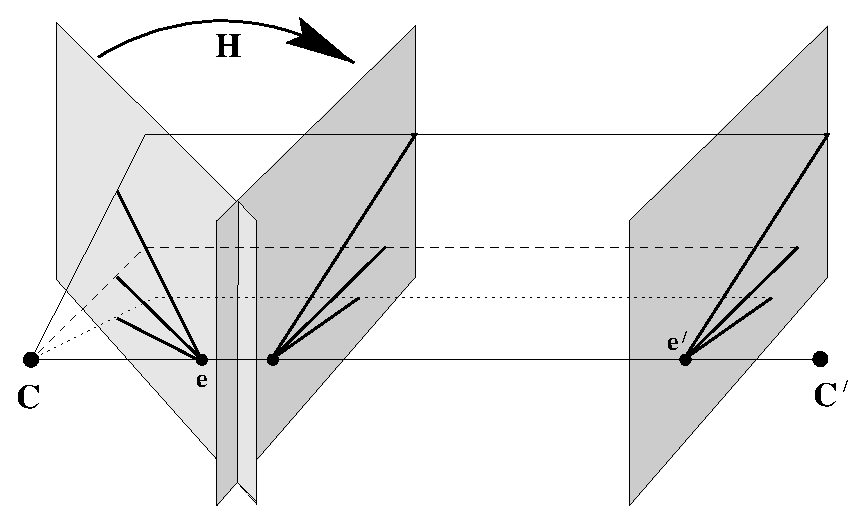
\includegraphics[scale=.5]{fig89}
  \caption{(Adapted from~\cite{Hartley2004}) The effect of the camera motion on
    the image points may be viewed as a two-step process: mapping by a
    homography $\mathrm{H_\infty}$ followed by a motion along the corresponding
    epipolar lines.}
  \label{fig:two_step_motion}
\end{figure}

In a general case the mapping of an image point $\mathbf{x}$ into
$\mathbf{x}'$ may be viewed as a two step process: transformation by a
homology (a specialization of homography which has two equal
eigenvalues) $\mathrm{H_\infty}$ which simulates a pure rotational
motion of the camera followed by an offset along the epipolar line
which simulates a pure translational motion of the camera, see Figure~\ref{fig:two_step_motion}.

\section{Motion Estimation}\label{sec:moest}

Our strategy to attack the problem is to separate it into two smaller
sub-problems: rotation estimation and translation estimation. The
algorithm relies on the ability to partition the scene points into two
sets: the distant and the near-by ones.  The distant points are used
for rotation estimation while the near-by ones take part in the
translation estimation.

First, the stereo algorithm is presented, followed by the monocular
one.  The main difference is in the translation estimation part. While
it is possible to implement a stereo-like algorithm in the monocular
setting as well, it suffers from the scale drift.  Thus, we propose a
different technique.


\subsection{Stereo}\label{sec:stereo_moest}
\paragraph{Partitioning the points} To partition the points in the
stereo case we hard-threshold their $Z$-coordinates (the threshold is
a parameter of the algorithm).  The depth of the points was computed
by a stereo triangulation.

\paragraph{Rotation Estimation:}\label{sec:rotation_estimation}
We use distant points to estimate rotation $\mathrm{R}$ (i.e., near-by
points do not take part in rotation estimation). As Eq.
(\ref{eq:general_point_motion}) states:

\begin{equation}
  \mathbf{x}' = \mathrm{KRK^{-1}}\mathbf{x} + \mathrm{K}\mathbf{t}/Z.
\end{equation}

The total motion of the feature point in the image plane may be viewed
as a two-step process (the order is not important): transformation by
homography $\mathrm{H_\infty} = \mathrm{KRK^{-1}}$ followed by
displacement along the line defined by the epipole $e'$ and the point
$\mathrm{H_\infty}\mathbf{x}$.  The magnitude of the displacement
along the epipolar line depends on the the camera translation and the
inverse depth of the point, see Figure~\ref{fig:feature_motion}.

\begin{figure}[h]
  \centering
  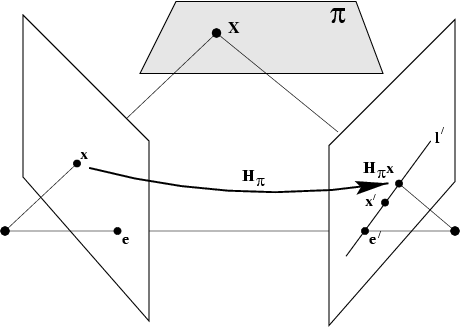
\includegraphics[scale=.5]{fig85_adapted}
  \caption{(Adapted from~\cite{Hartley2004}) The homography $H_\pi$ transfers the point onto a corresponding epipolar line.  The displacement along the epipolar line depends on the inverse depth of the point and the camera translation magnitude.}
  \label{fig:feature_motion}
\end{figure}                                                             %

Our estimation algorithm consists of initialization and non-linear
refinement.
\paragraph{Initialization:} to compute the initial estimate of the rotation
parameters we assume that for the distant points (s.t., $\norm{\mathbf{t}}/Z \ll \norm{\mathrm{H_\infty}\mathbf{x}}$):

\begin{equation}\label{eq:homography_transfer}
  \mathbf{x}' \approx \mathrm{KRK^{-1}}\mathbf{x}.
\end{equation}

This assumption is justified by the fact that for the distant points
the displacement along the epipolar line is small. We multiply
both sides of Eq. (\ref{eq:homography_transfer}) by $\mathrm{K^{-1}}$
and denote $\mathbf{u'} = \mathrm{K^{-1}}\mathbf{x}$ and
$\mathbf{u} = \mathrm{K^{-1}}\mathbf{x}$:

\begin{equation}
  \mathbf{u'} = \mathrm{K^{-1}}\mathbf{x}' \approx \mathrm{RK^{-1}}\mathbf{x} = \mathrm{R}\mathbf{u}.
\end{equation}

Since $\mathbf{u}$ and $\mathbf{u}'$ are projective quantities, only
their directions are of importance, we normalize them to unit length
and denote normalized quantities by $\mathbf{\tilde{u}}$ and
$\mathbf{\tilde{u}}'$ respectively. We choose a sample of $n$ points
($n=3$) and stack them as columns of matrices $\mathrm{\tilde{U}}$ and
$\mathrm{\tilde{U}'}$ respectively.  We search for $\mathrm{R}$ that
solves the following minimization problem:

\begin{equation}\label{eq:absolute_orientation}
\underset{\mathrm{R}}{\text{argmin}}\ \norm{\mathrm{\tilde{U}'-R\tilde{U}}}_2.
\end{equation}

Eq. (\ref{eq:absolute_orientation}) is known as the absolute
orientation problem (see e.g.,~\cite{Horn1987}) and its solution
provides an initial estimate for the subsequent non-linear
optimization problem.

\paragraph{Refinement:} The idea of the refinement is this: the
residual vector $\mathrm{H}_\infty\mathbf{x} - \mathbf{x}'$ may be
viewed as a sum of a vector orthogonal to the epipolar line and the
vector parallel to it.  We search for the camera rotation that ignores
the parallel component (we view it as a ``legal'' bias) while trying
to minimize the orthogonal one.  We define the point residual as the
orthogonal distance to the corresponding epipolar line and minimize
the sum of squared residuals for all points.  We do so, because, as
Eq. (\ref{eq:general_point_motion}) suggests, after we compensate for
a rotation, the point is still allowed to move along the epipolar
line.

Consider the objective:

\begin{equation}\label{eq:refinement_objective}
  \begin{split}
    \mathrm{R(v,\theta)} = \underset{v,\ \theta}{\mathrm{argmin}}
    \sum_{i=1}^N{r_i}^2\quad \text{s.t.}\quad r_i&=n_i\cdot (\mathbf{x}_i'-H_\infty(v,\theta)\mathbf{x}_i) \\
    \text{where}\ n_i &= (\mathrm{F}\mathbf{x}_i)_\perp
  \end{split}
\end{equation}
$\mathrm{H_\infty}(v,\theta) = \mathrm{KR(v,\theta)K^{-1}}$ is the
homography that transforms the image points in Eq.
(\ref{eq:general_point_motion}). It depends on a known camera
intrinsic matrices $\mathrm{K}$ and a rotation matrix $\mathrm{R}$.
We choose to parameterize the rotation by an angle $\theta$ and an
axis $v$.  $\mathrm{F}$ denotes the fundamental matrix that
corresponds to two subsequent stereo rig poses and is computed
elsewhere. $\mathrm{F}\mathbf{x}_i$ denotes the epipolar line that
corresponds to $\mathbf{x}_i$ in the second image and
$(\mathrm{F}\mathbf{x}_i)_\perp$ is the normal to this line.
We solve the minimization problem
(\ref{eq:refinement_objective}) by means of the Levenberg-Marquardt
optimization algorithm.

To make the estimation robust we wrap the initialization procedure
into the RANSAC iterations.  We choose the strongest consensus
estimate and its support set as an input for the solution of the
Eq. (\ref{eq:refinement_objective}).

\paragraph{Translation Estimation (1-point
  algorithm)}\label{sec:stereo_trans} To estimate
the translation we use only the near-by points.  First, we triangulate
these points in the previous stereo pair to obtain their 3-D
locations, and then iteratively minimize the sum of reprojection
errors into the current frame.

The reprojection of point $\mathbf{X}=(X,Y,Z,1)^T$ into the current
left image is given by:
\begin{equation}
  \pi^{(l)}(\mathbf{X};\mathbf{t}) =  K\Bigl[ \mathrm{R}\ |\ \mathbf{t} \Bigr]\mathbf{X}.
\end{equation}
and the reprojection of the same point into the current right image
($b$ is the baseline of the stereo-rig) is given by:
\begin{equation}
  \pi^{(r)}(\mathbf{X};\mathbf{t}) =  K\Bigl[ \mathrm{R}\ |\ \mathbf{t} \Bigr](\mathbf{X} - (b,0,0,0)^T),
\end{equation}

We use the Levenberg-Marquardt algorithm to iteratively minimize the
sum of squared reprojection errors (starting from
$\mathbf{t}=\mathbf{0}$):
\begin{equation}
\norm{\mathbf{x'} - \pi^{(l)}(\mathbf{X};\mathbf{t})}^2 + \norm{\mathbf{x'} - \pi^{(r)}(\mathbf{X};\mathbf{t})}^2.
\end{equation}

There are three unknown parameters, since
$\mathbf{t} = (t_x,t_y,t_z)^T$, thus a single 3-D point provides
enough constraints to determine $\mathbf{t}$.

\subsection{Mono}\label{sec:mono_moest}

The stereo setup has an advantage over the monocular one in the sense
that it provides the algorithm with more information (e.g., the
calibration and the additional image at each camera position).  These
advantages come at a price, e.g., the cameras need to be synchronized
and the computational resource requirements climb.  These make
monocular setups and the related algorithms more attractive.  In the
following section we present the version of our algorithm, adapted for
the monocular setup.

Given two sets of matching image points $\mathbf{x}_i, \mathbf{x}_i'$
from two subsequent frames $I_1, I_2$ respectively, we estimate the
camera motion between these frames. Similar to the stereo algorithm in
Section \ref{sec:stereo_moest} the algorithm first partitions the
points and then estimates the rotation followed by the estimation of
the translation direction (it is well known that the magnitude of the
camera translation is unavailable in the monocular setting).

\paragraph{Partitioning the points} \label{sec:mono_split} To estimate
the rotation of the camera as in the Eq. (\ref{sec:moest}), it is
required to partition the set of the image points into the distant
ones and the near-by ones.  While in the stereo setting we may
triangulate the points and threshold their depths, in the monocular
setting this can not be done.  This section proposes a method to
perform the aforementioned partition in the monocular setting.

Consider the subsequent images $I_1, I_2, I_3$ taken by a moving
camera at the locations $O_1,O_2$ and $O_3$ respectively. We assume
the image points $\mathbf{x}_i$ in $I_1$ are known to be distant
relative to the camera at $O_1$.  The magnitude of the camera
translation is small relative to the distant points depths, thus we
assume that these points are distant w.r.t.\ the camera at $O_2$ and
$O_3$ as well.  Some of these points will be lost in $I_3$, thus it is
desirable to known which of the points tracked from $I_2$ to $I_3$
(which are not part of $\mathbf{x}_i$'s) are distant (denote these by
$\mathbf{y}_j$).

The real baselines $t_1=\norm{O_1-O_2}$ and $t_2=\norm{O_2-O_3}$ are
unknown and thus we can not use them to obtain real depths of the
points.

We use the following procedure to classify the newly tracked points in
$I_2$ as distant:
\begin{enumerate}
\item Set $t_1=1$ and triangulate the distant points $\mathbf{x}_i$ to
  obtain the depths $Z_i$
\item Set $t_2=1$ and triangulate the points $\mathbf{y}_j$ to obtain
  the depths $Z_j$
\item Classify the point $y_j$ to be distant if
  $Z_j>\underset{i}{\text{min}}\ Z_i$.
\end{enumerate}

While the assumption $t_1 \approx t_2$ is acceptable for the KITTI
dataset, it may be improved on by computing the $t_1/t_2$ ratio (by
minimizing the reprojection errors of $\mathbf{x}_i$ into $I_3$,
similar to the translation estimation described in the Section
\ref{sec:stereo_trans}).

To initialize the monocular algorithm we may further assume that the
initial motion is a pure translation and thus the points with small
disparity are the distant ones (disparity being the magnitude of the
motion in the image plane).

\paragraph{Rotation Estimation} is exactly as in the Section 
\ref{sec:rotation_estimation}. Denote the estimated rotation by
$\mathrm{R}$ and the corresponding homography by $\mathrm{H}$.

\paragraph{Translation Estimation} is as follows. Compensate the
rotation by computing $\mathbf{y}_i = \mathrm{H_\infty}\mathbf{x}_i$.  We optimize over the location of
the epipole $e$ and minimize the orthogonal distances of the points to
their corresponding epipolar lines:

\begin{align}
  \underset{e}{\text{argmin}}\ \sum_i{d(l_i,\mathbf{y}_i)+d(l_i,\mathbf{x}_i')}\ \text{s.t.}\  d(e,l_i) & =0\ \text{while}\ l_i = \underset{l}{\text{argmin}}\ d(l,\mathbf{x}_i') + d(l,\mathbf{y}_i)
\end{align}

We define the epipolar line $l_i$ to be the line that passes through
the epipole and its distance to $\mathbf{x}_i'$ and $\mathbf{y}_i$ is
minimal. $d(l,\mathbf{x})$ denotes the distance from the line $l$ to
the point $\mathbf{x}$.  The epipole provides us with the translation
direction of the camera.

\section{Experimental Results}\label{sec:results}

\subsection{The Choice of Features}
We chose to evaluate our algorithm on the KITTI
dataset~\cite{Geiger2012}, which is a de-facto standard for the
visual odometry research works.

\paragraph{Feature Detector/Descriptor:} We use Harris
~\cite{Harris1988} corner detector. It is fast, well localized and
(most important) Harris corners are abundant in urban scenes we work
with. We detect corners in each new image and then match them to
obtain putative matches.  We tune sensitivity threshold of the
detector in such a way, that we are left with about five hundred
putative matches after matching and pruning.  We extract a square
patch of $7\times 7$ pixels centered at the corner point and use this
vector as feature descriptor.

We would like to point out that our method may be used with any
feature detector that would allow to match features across images. The
choice of feature detector should be viewed as a parameter to the
algorithm and mainly depends on the images at test.

\paragraph{Feature Matching:} We use sum-of-square differences (SSD)
of feature descriptors as a metric function when matching
features. For each feature we choose a single best match w.r.t. the
metric function in the other image. We employ a number of heuristics
to prune outliers:
\begin{itemize}
\item Reciprocity: features $a$ and $b$ match only if $a$ matches $b$
  and $b$ matches $a$
\item Epipolar constraint: we work with calibrated stereo pair.  When
  we match features across images of stereo pair, the search is
  one-dimensional, i.e., along the horizontal epipolar line.  This
  heuristic is not used when matching features across subsequent
  frames.
\item Chierality (visibility): also used when matching features across
  stereo pair images.  We triangulate the features to obtain the 3-D
  point and keep the match only if the 3-D point is visible in both
  cameras.
\item Circular match: similar to ~\cite{Geiger2011} we keep only those
  matches that form a circle.
\end{itemize}

\subsection{Experimental Results}

The Tables \ref{table:rot_err} and \ref{table:trans_err} present the
results of the experiments for the KITTI dataset. The columns denote
the number of the sequence.  The rows denote the algorithm: SS is the
baseline, HX is the stereo version of the algorithm, HG is the
monocular version.  The numbers are the mean error for the
corresponding sequence with the last column is the mean error for the
dataset. The error computation method is described
in~\cite{Geiger2012}.

\paragraph{Stereo} In this set of experiments we ran our algorithm in
its stereo mode as described in the Section \ref{sec:stereo_moest}.
Table \ref{table:rot_err} and \ref{table:trans_err} present the
rotation and the translation errors respectively in the row HX. The
columns marked bold are those that our algorithm outperforms the
baseline (on 9 of 11 sequences). The results show that our algorithm improves the
rotation results over the benchmark algorithm and successfully
competes with it in the translation estimation.

\paragraph{Mono} In an additional set of experiments we ran our
algorithm in a monocular mode. Monocular motion estimation lacks a
scale parameter. In order to compare the results we set the
scale of the translation to be that of the stereo algorithm.  Feature
point selection/partition was done without using any stereo
information and the motion estimation was done as explained in the
Section~\ref{sec:mono_moest}.

\section{Conclusions and Discussion}
This paper presents a novel visual odometry algorithm.  The novelty of
the algorithm is in its rotation estimation method.  The rotation is
estimated by means of the infinite homography.  The algorithm may be
used both in the stereo and in the monocular setting.

The strengths of the presented algorithm are in its ability to split
the motion estimation problem into two smaller problems and to operate
directly on the image points instead of on the computed 3-D
quantities.  Splitting the problem helps because each sub-problem is
easier to solve.  The ability to partition the points into the distant
and the near-by ones is what allows us to separate the rotation and
the translation estimation.  

The stereo version of the algorithm shows better performance, but the
monocular version has the advantage of being a more practical one.
Indeed the authors in~\cite{Geiger2012} report that they re-calibrate
the cameras before each drive, which is hardly possible in real world
installations.

\begin{table}
  \centering
  \caption{Rotation errors for the KITTI sequences [deg/m]}
  \label{table:rot_err}
  \smallskip\noindent
  \resizebox{\linewidth}{!}{%
    \begin{tabular}{|c|c|c|c|c|c|c|c|c|c|c|c|c|}
\hline
 & 00 & 01 & 02 & 03 & 04 & 05 & 06 & 07 & 08 & 09 & 10 & mean \\
\hline
SS & 3.95e-04 & 1.98e-04 & 4.11e-04 & 1.07e-03 & 8.03e-04 & 3.49e-04 & 4.72e-04 & 2.96e-04 & 3.69e-04 & 3.44e-04 & 4.82e-04 & 4.71e-04 \\
\hline
HX & \textbf{2.70e-04} & \textbf{1.75e-04} & \textbf{4.10e-04} & \textbf{6.51e-04} & \textbf{6.04e-04} & 3.95e-04 & \textbf{3.77e-04} & \textbf{2.37e-04} & \textbf{3.23e-04} & \textbf{3.22e-04} & 5.66e-04 & \textbf{3.93e-04} \\
\hline
HG & 8.72e-04 & 3.89e-04 & 6.28e-04 & 1.07e-03 & 5.99e-04 & 6.96e-04 & 3.31e-04 & 8.12e-04 & 8.13e-04 & 6.82e-04 & 5.23e-04 & 6.74e-04 \\

\hline
\end{tabular}

  }
\end{table}

\begin{table}
  \centering
  \caption{Translation errors for the KITTI sequences \% }
  \label{table:trans_err}
  \smallskip\noindent
  \resizebox{\linewidth}{!}{%
    \centering
\begin{tabular}{|c|c|c|c|c|c|c|c|c|c|c|c|c|}
\hline
 & 00 & 01 & 02 & 03 & 04 & 05 & 06 & 07 & 08 & 09 & 10 & mean \\
\hline
SS & 4.40e+00 & 9.25e+00 & 4.03e+00 & 1.22e+01 & 5.06e+00 & 2.80e+00 & 4.37e+00 & 2.21e+00 & 4.12e+00 & 5.25e+00 & 5.60e+00 & 5.39e+00 \\
\hline
HX & 3.07e+00 & 1.08e+01 & 3.80e+00 & 7.94e+00 & 3.82e+00 & 4.06e+00 & 3.99e+00 & 1.67e+00 & 3.28e+00 & 3.77e+00 & 5.65e+00 & 4.72e+00 \\
\hline
HG & 1.21e+01 & 1.48e+01 & 8.72e+00 & 1.33e+01 & 8.62e+00 & 8.37e+00 & 4.46e+00 & 7.93e+00 & 9.76e+00 & 1.16e+01 & 8.36e+00 & 9.82e+00 \\
\hline
\end{tabular}

  }
\end{table}

\chapter{Monocular Scale}

\section{Introduction}

Recovering camera 6-DOF ego-motion from images is a well studied
problem. It arises in various practical contexts
(e.g. virtual/augmented reality application, autonomous or aided
navigation, etc.).  The problem was studied in both stereo and the
monocular setups.  To recover the full 6-DOF motion, the previous
works resorted to the stereo setup, used auxiliary sensors (e.g. IMU)
or made assumptions about the camera pose and the scene.  All of these
have their drawbacks: stereo pairs are fragile and require careful
calibration procedures, additional sensors are not always available
and also require calibration, scene assumptions don't always hold.
Motion estimation from images of a single moving camera is probably
the hardest setup, as well as the most desirable one, because of its
simplicity.  It is well known that the translation scale parameter is
not directly observable for a motion of a single camera.

We argue, that for natural scenes the scale information is present in
the images and may be extracted.  Our method learns a regressor, that
is capable to prediction the motion scale.

\section{Related work}
\paragraph{Geometry based methods} One category of works proceed by
making assumptions on the camera motion,
e.g.,~\cite{scaramuzza2009absolute}.  The authors assume that the
vehicle adheres to the Ackerman steering principle and exploit the
non-holomicity of the vehicle motion, to compute the exact scale of
the camera motion.  Other works make assumptions about the scene
(e.g., a presence of the planar surface in front of the vehicle) and
the height of the camera, e.g.~\cite{zhou2016reliable}, where the
authors estimate the ground plane homography that relates subsequent
images.  The motion scale is estimated/refined based on the homography
that relates the ground plane in subsequent images.
\paragraph{Learning methods} We are not aware of works that learn the
scale, rather there are a number of methods that use machine learning
approaches to tackle the visual odometry.  One such work
is~\cite{wang2017deepvo} that trains LSTM to predict the full 6-DOF
motion of the camera over sequences of
images. In~\cite{muller20017flowdometry} the authors use optical flow
images as CNN input to learn and infer camera motion. Authors
in~\cite{DBLP:journals/corr/MohantyADGSC16} also propose to train a
CNN.



\subsection{Our method}

We assume that a single camera moves through space and takes images.
We treat the initial camera pose (at time $t=0$) as the world
coordinate frame.  We denote the pose of the camera at time $t$ by
$\mathbf{\hat{T}}_t$ described by the rotation matrix
$\mathbf{\hat{R}}_t$ and the translation vector $\mathbf{\hat{t}}_t$
as seen in the world coordinate frame.  We denote camera image taken
at time $t$ by $I_t$.  To facilitate the discussion, we also introduce
notation for camera pose
$\mathbf{T}_t = [\mathbf{R}_t\ |\ \mathbf{t}_t] $ as seen from the
coordinate frame associated with camera pose at time $t-1$.  Most of
the time, we will omit the time index, since its clear from the
context.  By translation scale (or simply, scale) we refer to the norm
of the translation vector $\mathbf{t}$ (e.g.,
$s = \lVert \mathbf{t} \rVert$)

We pose the scale estimation problem as a regression problem and
search for a good regressor model.

\section{Random forest}

\subsection{Decision trees}

In this section we briefly describe tree-based methods for regression.
These involve splitting the feature space into a number of small
regions.  The prediction for a sample is made by computing a mean or a
mode of training samples that belong to the same region.  Since the
set of rules used to split the feature space into smaller regions may
be described by a tree, these methods are referred to as
\textit{decision tree} methods.

Building a decision tree may be described by a two step procedure:
\begin{enumerate}
\item Split the feature space, e.g., the set of all possible values
  for $X_1, X_2,\ldots,X_n$ into $J$ distinct regions $R_1, R_2,\ldots, R_J$.
\item For every sample that belongs to the regions $R_i$ we make the
  same prediction, which is a mean of the responses of training
  samples that belong to this region.
\end{enumerate}

The regions $R_i$ are usually chosen to be multidimensional boxes (axis aligned).  We would like to find such a partition of the feature space that minimizes
\begin{equation}\label{eq:tree_objective}
\sum\limits_{j=1}^J\sum_{x\in R_j}{(x-\mean{x}_j)^2}
\end{equation}

Where $\mean{x}_j$ denotes the mean of the response values of the
samples in region $R_j$.  Unfortunately, solving the optimization
problem~\ref{eq:tree_objective} is computationally hard.  Usually it
is replaced with a greedy algorithm, called \textit{recursive binary
  splitting}.  This approach starts at the top of the tree and
greedily chooses the best split at that point that minimizes the
variance of its sub-trees.  To be more precise, for each $j$ and $s$ we
define the hyper-planes:

\begin{equation}
  R_1(j,s) = \{ X\lvert X_j<s \}\quad\text{and}\quad R_2(j,s) = \{ X\lvert X_j \geq s \},
\end{equation}

We seek such $j$ and $s$ that minimize the equation:

\begin{equation}
  \sum\limits_{i:x_i\in R_1(j,s)}{(y_i-\hat{y}_{R_1})}^2 + \sum\limits_{i:x_i\in R_2(j,s)}{(y_i-\hat{y}_{R_2})}^2,
\end{equation}

Where $y_{R_1}, y_{R_2}$ are the average responses of the samples in
$R_1(j,s), R_2(j,s)$ respectively.  Once we found the $j$ and $s$ we
recursively split each sub-tree in a similar manner.  The process is
repeated until a stopping criterion (e.g., number of nodes in the
leaf) is reached.

\subsection{Bagging}
Decision trees tend to suffer from \textit{high variance}. This means
that if we split the training set into a number of random subsets and
fit random tree into each sub-sample, we would likely to get much
different answers from these trees when asked the same question.  It
is known that the variance of a mean of a set of independent random
variables is $\frac{1}{n}$.  Thus, in order to improve the variance of
the estimator, it is possible to fit $n$ estimators, each to its
training-set and the average their predictions.  Since, usually, we
don't have $n$ training sets, we would use \textit{bootstrapping}
(e.g., sample independently with replacement from the data set).

\subsection{Random Forest}
The random forest suggests an additional improvement over bagging, by
decorrelating the random trees.  The issue they attempt to address is
this: lets say there is a very dominant feature w.r.t. to task at hand
for a given data-set.  Bagging ensures that we use different training
sets, but yet, most trees will tend to first split on this dominant
feature.  In this case the trees will resemble each other.  In random
forest, the trees are constructed by using only a subset of features
(e.g., $m = \sqrt{p}$).  This means that at calculating the splits,
the algorithm is allowed to consider only a subset of features.

\section{Convolutional Neural Networks}

Convolutional neural networks (CNN) leverage the availability of the
computational power and the abundance of data.  CNN have become a
method of choice in a number of computer vision areas (e.g., image
classification~\cite{krizhevsky2012imagenet} ~\cite{simonyan2014very},
~\cite{szegedy2015going}, object recognition
~\cite{sermanet2013overfeat}~\cite{girshick2014rich}
~\cite{he2014spatial}.  They were also shown capable of per-pixel
tasks, such as semantic segmentation
~\cite{ning2005toward}~\cite{gupta2014learning}, depth estimation from
a single image ~\cite{liu2016learning}, optical flow
estimation~\cite{fischer2015flownet}.

Network architecture is a choice that needs to be made a priori.  To
best of our knowledge, there is no clear guideline on how to choose a
network architecture for a new task.  We experiment with two network architectures:

\begin{itemize}
\item the ZF~\cite{DBLP:journals/corr/ZeilerF13} object recognition
  network.  This is a more traditional CNN architecture.
\item the FlowNet~\cite{fischer2015flownet} optical flow estimation
  network.  This architecture adheres to a newer fully-convolutional
  family of networks.  These are known to train better and have less
  parameters vs. their fully-connected counterpart networks.
\end{itemize}

The input to our network is a pair of subsequent images.  A decision
to make is how to input the images into the network.  There are two
common choices: either create two siamese branches, so that each gets
its own input image, or to create a single multi-channel image.
~\cite{fischer2015flownet} show that the latter works equally well
while being simpler, so we choose to concatenate the images along the
channel dimension to produce a single 6-channel (for color) or
2-channel (for gray-scale) image.

\subsection{ZF}

The network architecture consists of five convolutional and three fully connected layers.  Table~\ref{tab:zf_geometry} summarizes the architecture.

\begin{table}[ht]
  \begin{tabular}{lcccc}
    \toprule
    \textbf{Layer} & \textbf{Receptive Field Size} & \textbf{Padding} & \textbf{Stride} & \textbf{Number of Channels}\\
    \midrule
    conv1&  $7\times 7$& 2& 3&   96\\
    conv2&  $5\times 5$& 2& 2&  256\\
    conv3&  $3\times 3$& 1& 1&  384\\
    conv4&  $3\times 3$& 1& 1&  384\\
    conv5&  $3\times 3$& 1& 1&  256\\
    fc6&               &  &  & 4096\\
    fc7&               &  &  & 4096\\
    fc8&               &  &  &    1\\
  \end{tabular}
  \caption{ZF network geometry}
  \label{tab:zf_geometry}
\end{table}

The flow of data through the network
\begin{figure}
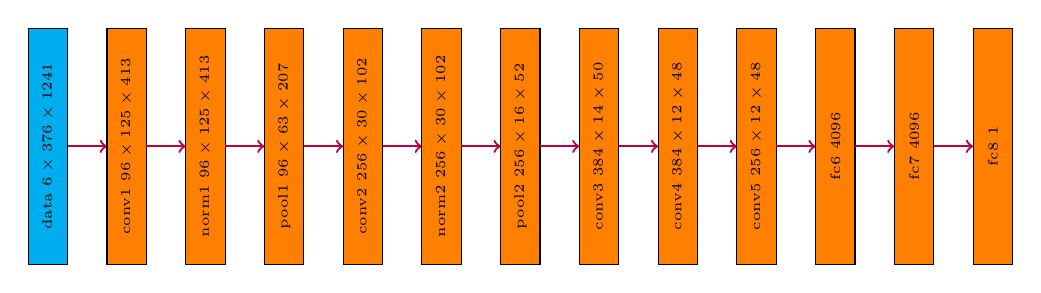
\begin{tikzpicture}
\draw[fill=cyan] (1.0, 0) rectangle (1.5, 3.0);
\draw[->, thick, purple] (1.5, 1.5) --(2.0, 1.5);
\node[font=\tiny, rotate=90] at (1.25, 1.5) {data $6\times 376\times 1241$};
\draw[fill=orange] (2.0, 0) rectangle (2.5, 3.0);
\draw[->, thick, purple] (2.5, 1.5) --(3.0, 1.5);
\node[font=\tiny, rotate=90] at (2.25, 1.5) {conv1 $96\times 125\times 413$};
\draw[fill=orange] (3.0, 0) rectangle (3.5, 3.0);
\draw[->, thick, purple] (3.5, 1.5) --(4.0, 1.5);
\node[font=\tiny, rotate=90] at (3.25, 1.5) {norm1 $96\times 125\times 413$};
\draw[fill=orange] (4.0, 0) rectangle (4.5, 3.0);
\draw[->, thick, purple] (4.5, 1.5) --(5.0, 1.5);
\node[font=\tiny, rotate=90] at (4.25, 1.5) {pool1 $96\times 63\times 207$};
\draw[fill=orange] (5.0, 0) rectangle (5.5, 3.0);
\draw[->, thick, purple] (5.5, 1.5) --(6.0, 1.5);
\node[font=\tiny, rotate=90] at (5.25, 1.5) {conv2 $256\times 30\times 102$};
\draw[fill=orange] (6.0, 0) rectangle (6.5, 3.0);
\draw[->, thick, purple] (6.5, 1.5) --(7.0, 1.5);
\node[font=\tiny, rotate=90] at (6.25, 1.5) {norm2 $256\times 30\times 102$};
\draw[fill=orange] (7.0, 0) rectangle (7.5, 3.0);
\draw[->, thick, purple] (7.5, 1.5) --(8.0, 1.5);
\node[font=\tiny, rotate=90] at (7.25, 1.5) {pool2 $256\times 16\times 52$};
\draw[fill=orange] (8.0, 0) rectangle (8.5, 3.0);
\draw[->, thick, purple] (8.5, 1.5) --(9.0, 1.5);
\node[font=\tiny, rotate=90] at (8.25, 1.5) {conv3 $384\times 14\times 50$};
\draw[fill=orange] (9.0, 0) rectangle (9.5, 3.0);
\draw[->, thick, purple] (9.5, 1.5) --(10.0, 1.5);
\node[font=\tiny, rotate=90] at (9.25, 1.5) {conv4 $384\times 12\times 48$};
\draw[fill=orange] (10.0, 0) rectangle (10.5, 3.0);
\draw[->, thick, purple] (10.5, 1.5) --(11.0, 1.5);
\node[font=\tiny, rotate=90] at (10.25, 1.5) {conv5 $256\times 12\times 48$};
\draw[fill=orange] (11.0, 0) rectangle (11.5, 3.0);
\draw[->, thick, purple] (11.5, 1.5) --(12.0, 1.5);
\node[font=\tiny, rotate=90] at (11.25, 1.5) {fc6 $4096$};
\draw[fill=orange] (12.0, 0) rectangle (12.5, 3.0);
\draw[->, thick, purple] (12.5, 1.5) --(13.0, 1.5);
\node[font=\tiny, rotate=90] at (12.25, 1.5) {fc7 $4096$};
\draw[fill=orange] (13.0, 0) rectangle (13.5, 3.0);
\node[font=\tiny, rotate=90] at (13.25, 1.5) {fc8 $1$};
\end{tikzpicture}
\caption{ZF network data flow.  Each rectangle depicts a top blob for a corresponding layer.}
\end{figure}

There is a last fully connected layer that reduces a network to a
single output, which we are interested to learn.  We use euclidean
loss to train the network.  Total number of parameters is about 624
million.


\subsection{FlowNet}

Fully-convolutional network is a recent trend in the field.  They are
known to train better and have less parameters vs. their fully
connected counterparts~\cite{long2015fully}. The geometry of the
network is described in Table~\ref{tab:flownet_geometry}. Each
convolutional layer is followed by the non-linearity.  We chose this
architecture since it proved successful for optical flow estimation
task and has pre-trained model readily available.

\begin{table}[ht]
  \begin{tabular}{lcccc}
    \toprule
    \textbf{Layer} & \textbf{Receptive Field Size} & \textbf{Padding} & \textbf{Stride} & \textbf{Number of Channels}\\
    \midrule
    conv1&   $7\times 7$& 3& 2&   64\\
    conv2&   $5\times 5$& 2& 2&  128\\
    conv3&   $5\times 5$& 2& 2&  256\\
    conv3-1& $3\times 3$& 1& 1&  256\\
    conv4&   $3\times 3$& 1& 2&  512\\
    conv4-1& $3\times 3$& 1& 1&  512\\
    conv5&   $3\times 3$& 1& 2&  512\\
    conv5-1& $3\times 3$& 1& 1&  512\\
    conv6&   $3\times 3$& 1& 2& 1024\\
    conv6-1& $3\times 3$& 1& 1& 1024\\
    conv7&   $3\times 3$& 1& 2&    1\\
    \hline
  \end{tabular}
  \caption{Geometry of the FlowNet based network}
  \label{tab:flownet_geometry}
\end{table}

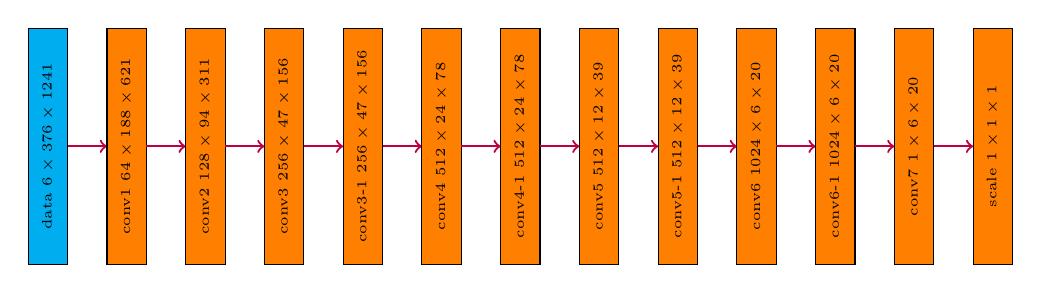
\begin{tikzpicture}
\draw[fill=cyan] (1.0, 0) rectangle (1.5, 3.0);
\draw[->, thick, purple] (1.5, 1.5) --(2.0, 1.5);
\node[font=\tiny, rotate=90] at (1.25, 1.5) {data $6\times 376\times 1241$};
\draw[fill=orange] (2.0, 0) rectangle (2.5, 3.0);
\draw[->, thick, purple] (2.5, 1.5) --(3.0, 1.5);
\node[font=\tiny, rotate=90] at (2.25, 1.5) {conv1 $64\times 188\times 621$};
\draw[fill=orange] (3.0, 0) rectangle (3.5, 3.0);
\draw[->, thick, purple] (3.5, 1.5) --(4.0, 1.5);
\node[font=\tiny, rotate=90] at (3.25, 1.5) {conv2 $128\times 94\times 311$};
\draw[fill=orange] (4.0, 0) rectangle (4.5, 3.0);
\draw[->, thick, purple] (4.5, 1.5) --(5.0, 1.5);
\node[font=\tiny, rotate=90] at (4.25, 1.5) {conv3 $256\times 47\times 156$};
\draw[fill=orange] (5.0, 0) rectangle (5.5, 3.0);
\draw[->, thick, purple] (5.5, 1.5) --(6.0, 1.5);
\node[font=\tiny, rotate=90] at (5.25, 1.5) {conv3-1 $256\times 47\times 156$};
\draw[fill=orange] (6.0, 0) rectangle (6.5, 3.0);
\draw[->, thick, purple] (6.5, 1.5) --(7.0, 1.5);
\node[font=\tiny, rotate=90] at (6.25, 1.5) {conv4 $512\times 24\times 78$};
\draw[fill=orange] (7.0, 0) rectangle (7.5, 3.0);
\draw[->, thick, purple] (7.5, 1.5) --(8.0, 1.5);
\node[font=\tiny, rotate=90] at (7.25, 1.5) {conv4-1 $512\times 24\times 78$};
\draw[fill=orange] (8.0, 0) rectangle (8.5, 3.0);
\draw[->, thick, purple] (8.5, 1.5) --(9.0, 1.5);
\node[font=\tiny, rotate=90] at (8.25, 1.5) {conv5 $512\times 12\times 39$};
\draw[fill=orange] (9.0, 0) rectangle (9.5, 3.0);
\draw[->, thick, purple] (9.5, 1.5) --(10.0, 1.5);
\node[font=\tiny, rotate=90] at (9.25, 1.5) {conv5-1 $512\times 12\times 39$};
\draw[fill=orange] (10.0, 0) rectangle (10.5, 3.0);
\draw[->, thick, purple] (10.5, 1.5) --(11.0, 1.5);
\node[font=\tiny, rotate=90] at (10.25, 1.5) {conv6 $1024\times 6\times 20$};
\draw[fill=orange] (11.0, 0) rectangle (11.5, 3.0);
\draw[->, thick, purple] (11.5, 1.5) --(12.0, 1.5);
\node[font=\tiny, rotate=90] at (11.25, 1.5) {conv6-1 $1024\times 6\times 20$};
\draw[fill=orange] (12.0, 0) rectangle (12.5, 3.0);
\draw[->, thick, purple] (12.5, 1.5) --(13.0, 1.5);
\node[font=\tiny, rotate=90] at (12.25, 1.5) {conv7 $1\times 6\times 20$};
\draw[fill=orange] (13.0, 0) rectangle (13.5, 3.0);
\node[font=\tiny, rotate=90] at (13.25, 1.5) {scale $1\times 1\times 1$};
\end{tikzpicture}

We use Euclidean loss to train the network. The total number of
parameters is 24 million.

\section{Recurrent Neural Networks}

Many problems require passing information through time.  Since the
traditional neural networks are stateless, they are poorly suited for
this purpose. Recurrent Neural Networks have loops in them, so that
the information can persist.

\begin{figure}[h!]
  \centering 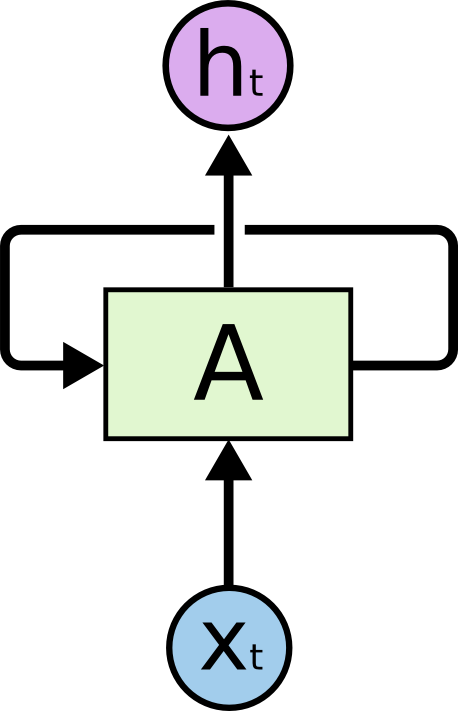
\includegraphics[width=0.15\textwidth]{RNN-rolled}
  \caption{RNN}
  \label{fig:rnn1}  
\end{figure}

In the Figure~\ref{fig:rnn1} network $A$ accepts input $x_t$ and
outputs $h_t$.  The loop allows the network to pass information from
one step of to another.

The RNN may be thought of as a chain of multiple copies of the same
neural network where each node passes a message to its successor.
This is called \textit{network unrolling}, depicted in
Figure~\ref{fig:rnn2}.  Unrolled network stresses the relation of the
RNN to the sequential data streams.  This is an architecture of choice
when modeling such data.

\begin{figure}[ht!]
  \centering 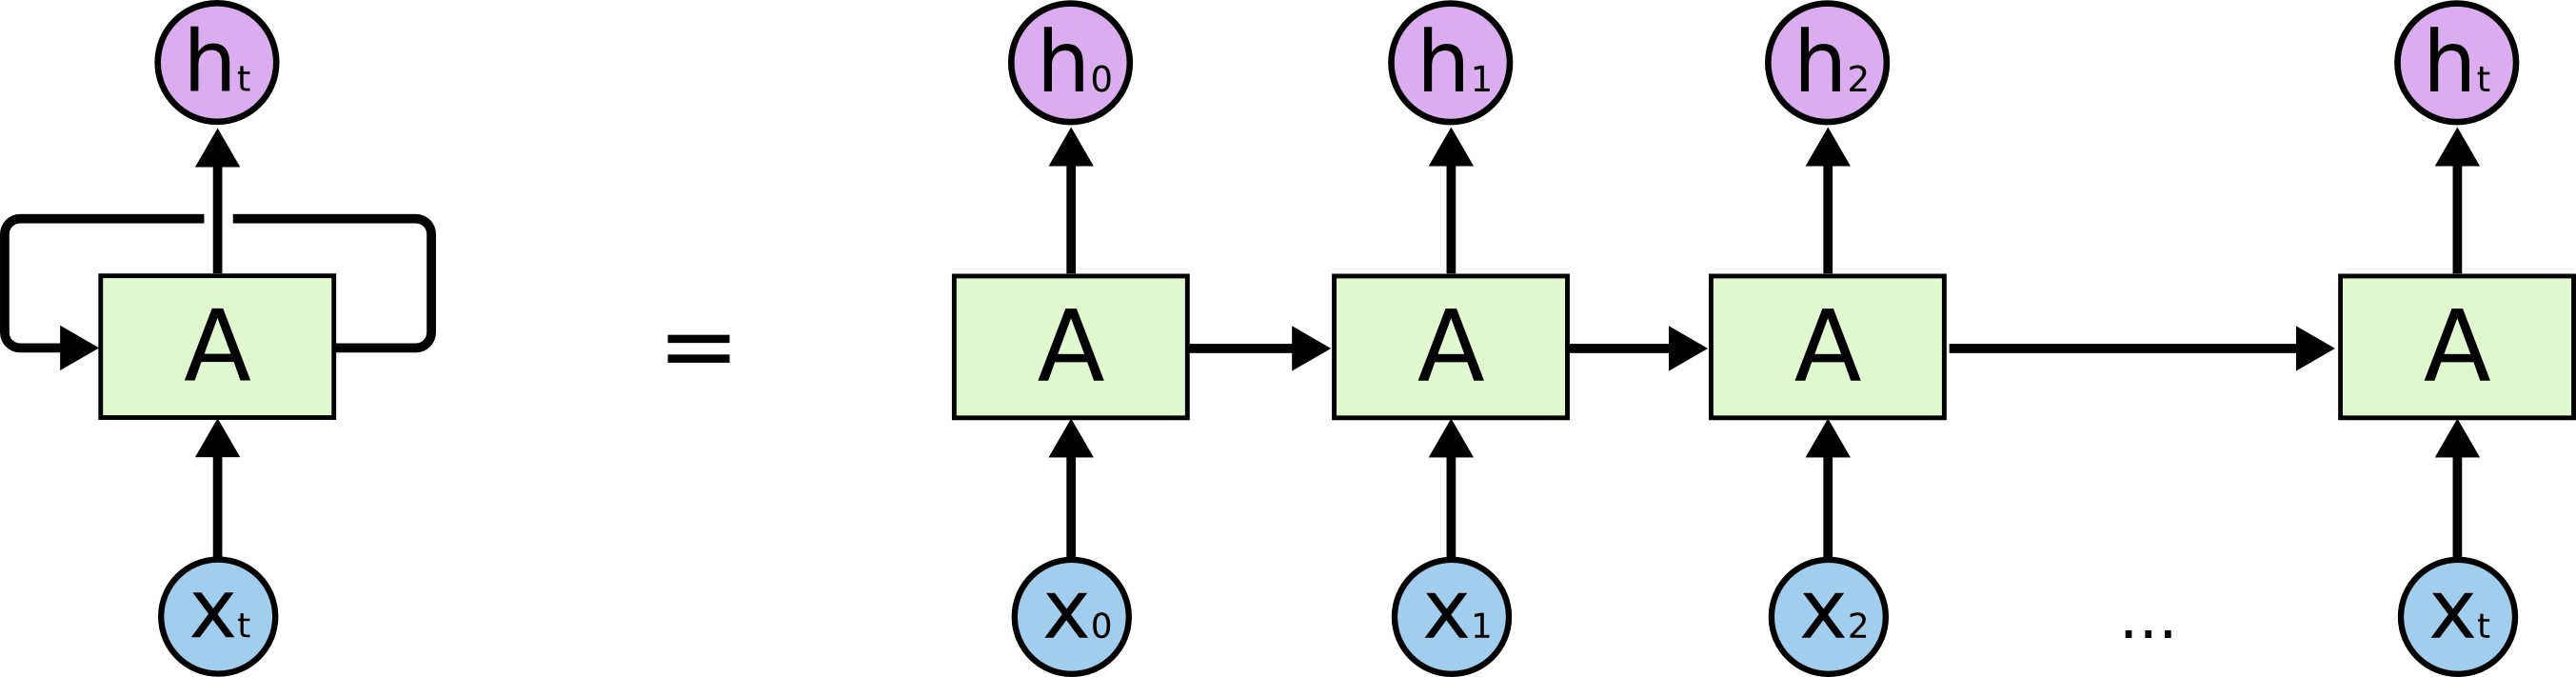
\includegraphics[width=.7\textwidth]{RNN-unrolled}
  \caption{An unrolled RNN}\label{fig:rnn2}
\end{figure}

It turns out that the vanilla RNN are hard to train due to the
exploding/imploding gradients.  Fortunately, Long Short Term Memory
Networks (LSTM), which is a special kind of RNN addresses these issues.

LSTM were introduced by~\cite{hochreiter1997long}, they are
specifically designed to model long term dependencies. Similarly to
RNN, LSTM posses a chain-like structure. Each repeating node has an
internal structure depicted in Figure~\ref{fig:lstm1}.

\begin{figure}[ht!]
  \centering 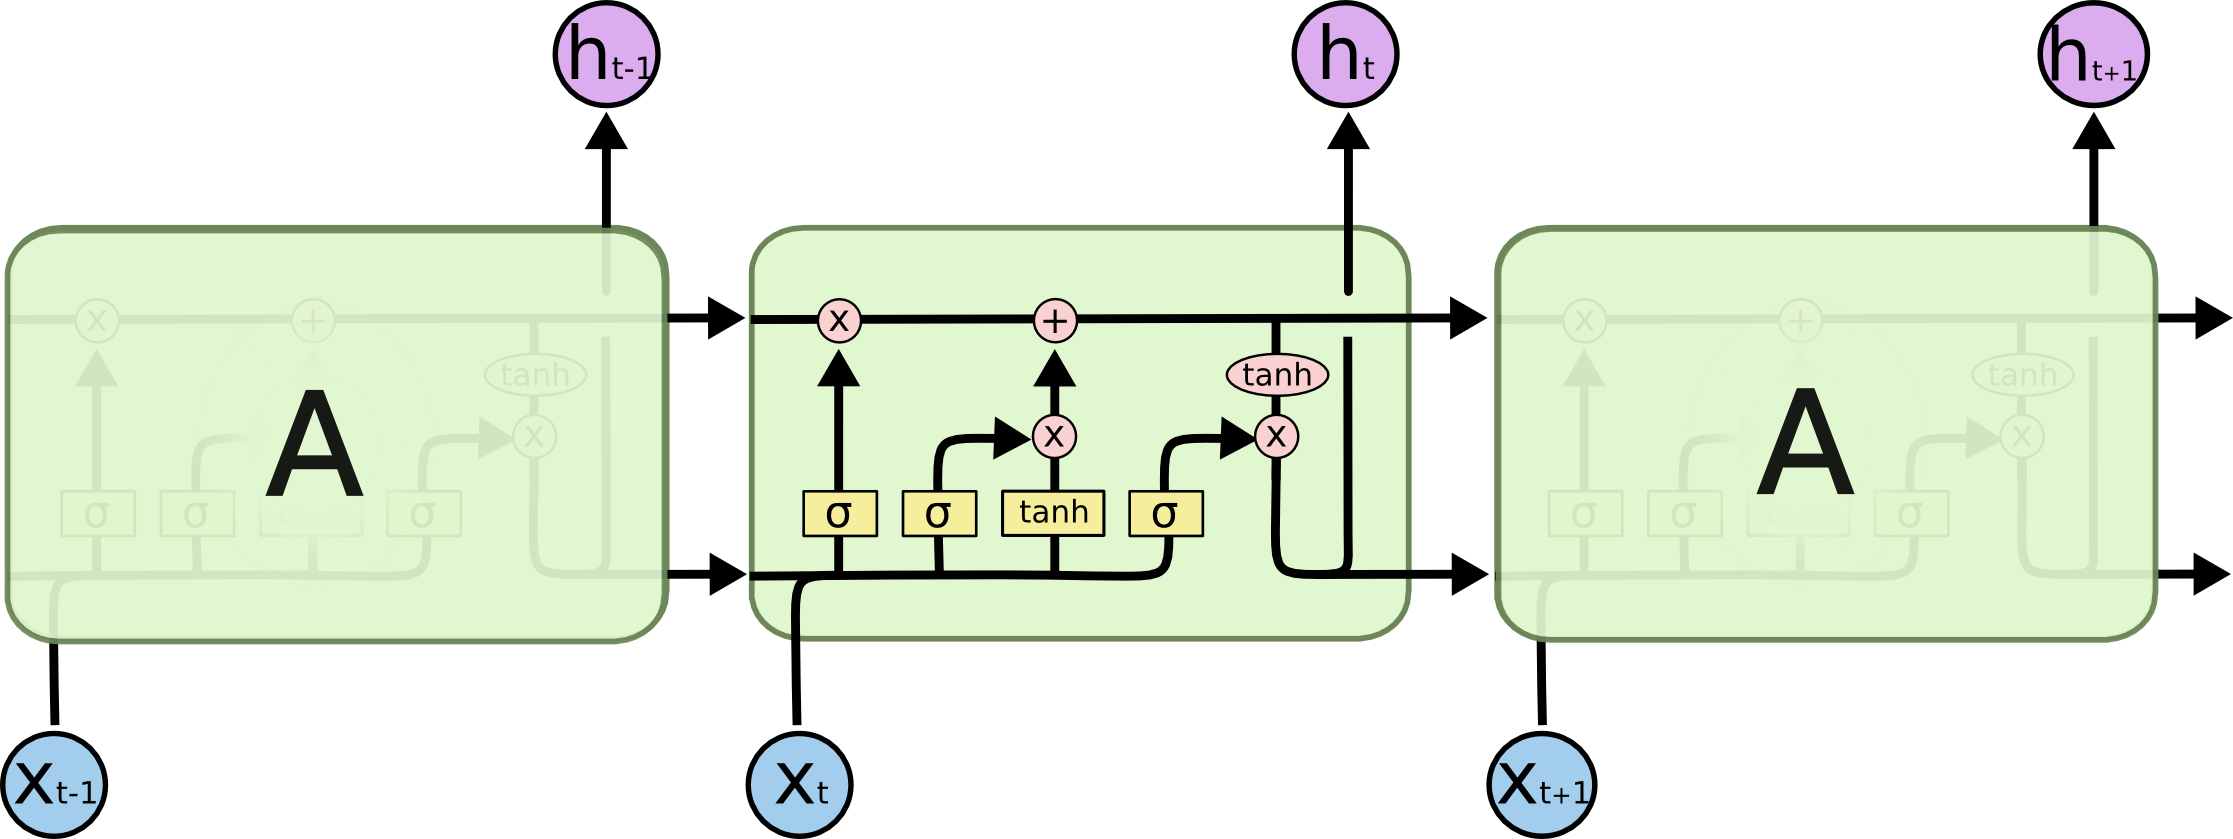
\includegraphics[width=.7\textwidth]{LSTM3-chain}
  \caption{Long Short Term Memory}\label{fig:lstm1}
\end{figure}

\begin{figure}[ht!]
  \centering 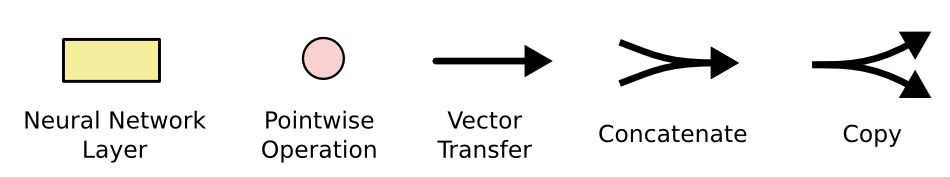
\includegraphics[width=.5\textwidth]{LSTM2-notation}
  \caption{A notation used in Figure~\ref{fig:lstm1}}\label{fig:lstm2}
\end{figure}

To use the LSTM for the image data we combine the convolutional
network with the LSTM.  $X_t$ vectors are produced by the ZF convnet.
This is a fairly common representation used previously.  The convnet
and the LSTM are trained jointly.

The geometry of the network is as follows:
\begin{itemize}
\item conv1: (96, 6, 7, 7)
\item conv2: (384, 48, 5, 5)
\item conv3: (512, 384, 3, 3)
\item conv4: (512, 256, 3, 3)
\item conv5: (384, 256, 3, 3)
\item fc6:   (4096, 34560)
\item lstm1: (1024, 4096)
\item fc-final: (1, 256)
\end{itemize}
Total number of trainable parameters is about 150 millions.

\section{Experiments}

\subsection{Data-set}

We train and test on the KITTI data-set~\cite{geiger2013vision}.  The
data-set consists of 11 sequences with ground truth data.  We
arbitrarily use sequence 00 for testing and sequences 01-10 for
training.  There are 4540 and 18650 images in the test and the train
sets respectively. We only use the data from the left color camera.
Figure~\ref{fig:scales} depicts the distribution of the scale values
over the train and the test sets.

\begin{figure}[!ht]
  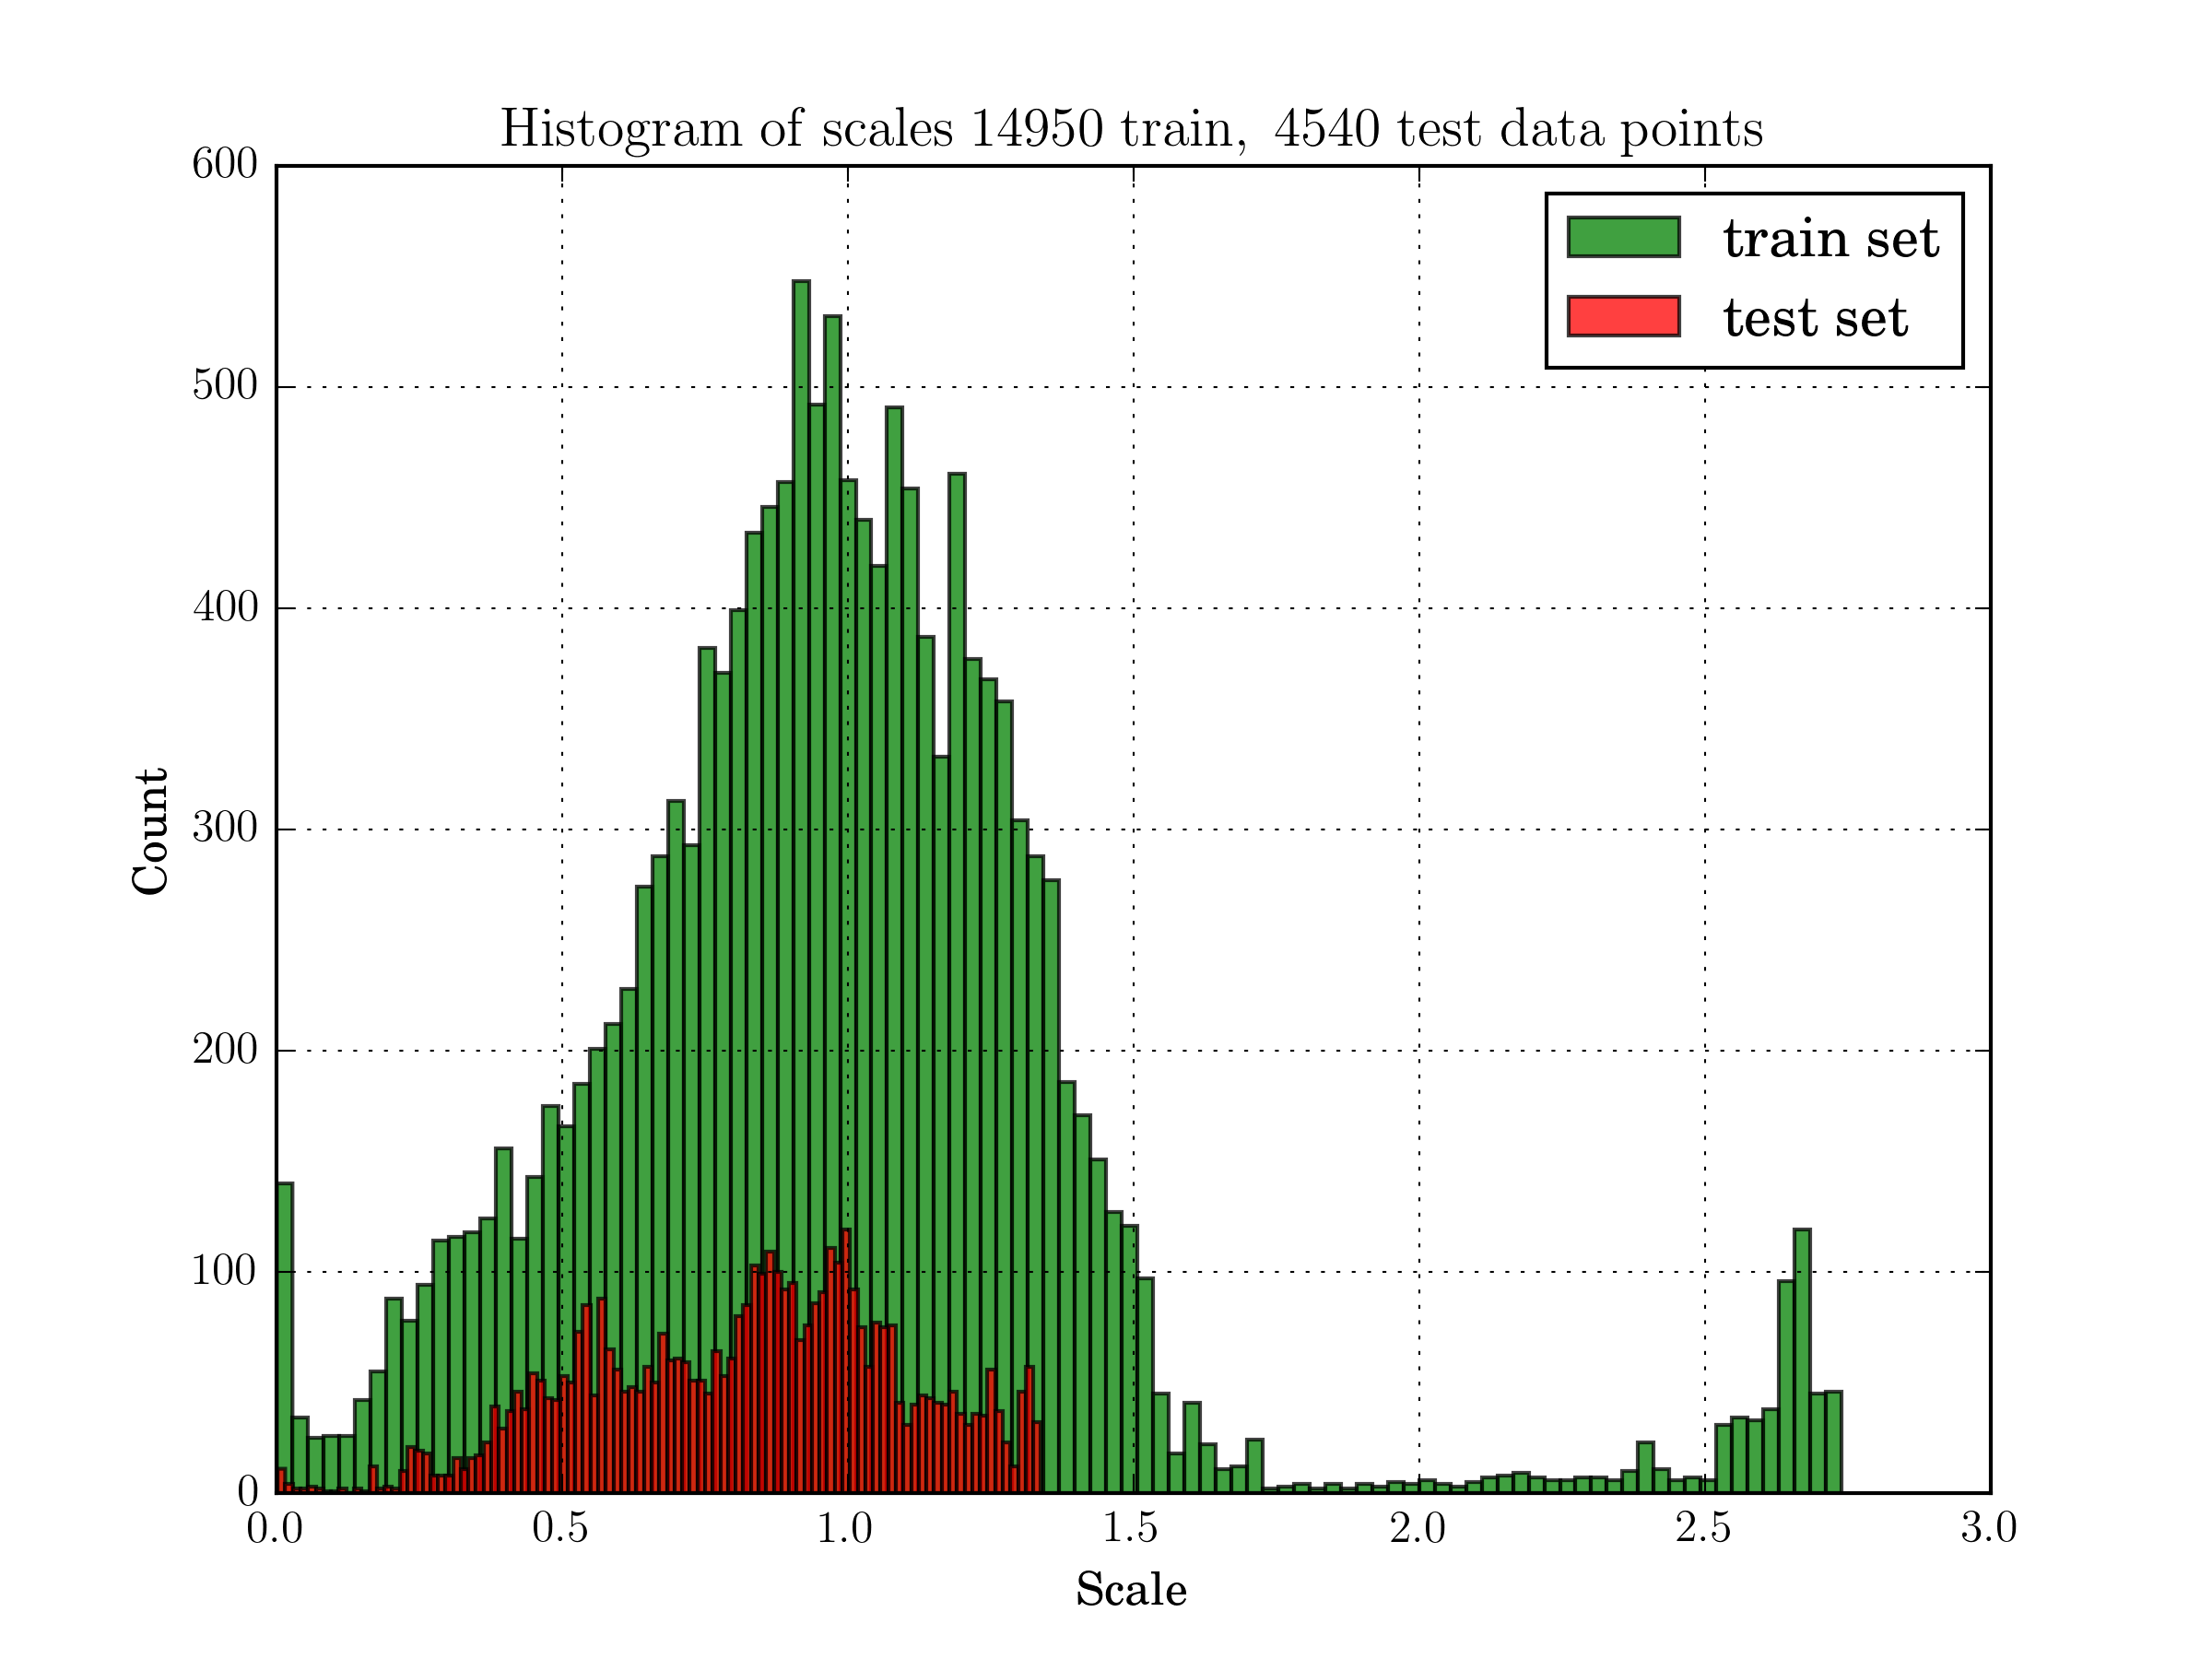
\includegraphics[width=0.9\linewidth]{no_00-scales}
  \caption{The train set}
  \label{fig:stats-no_00}
  \caption{Scale distributions}
  \label{fig:scales}
\end{figure}

\subsection{Random Forest}

\subsection{Feature Extraction}\label{sec:features}

In order to train the random forest we need to represent subsequent
image pairs as feature vectors, which are created as follows: we
extract and match sparse salient points in both input images.  The
output of this stage is a set of a corresponding pixel locations.
Then, we compute the point displacement magnitudes.  Finally, we bin
all the interest pundits according to a grid and create histogram of
displacement magnitudes for each bin.  Concatenating all histograms
together produces a feature vector. We use Harris corners and square
$11\times 11$ patches as corner descriptors. Sum of square differences
is used as a distance measure with the winning pair declared a match.
To prune the outliers we fit the fundamental matrix into the matched
corner sets and remove the corners that do not agree with the model.
Figure~\ref{fig:ex_corner_and_matching} shows a typical example of
extracted and matched corners.


Some statistics of the features is presented in the
Figure~\ref{fig:feature_vectors}. We expect the peaks, that correspond
to a closer image regions have a distributions shifted to the right
(i.e., larger displacements) and the peaks that correspond to a
regions farther away should be closer to zero.  This behavior can be
observed especially well for the feature vectors that correspond to
larger camera displacements (e.g. Figure~\ref{fig:1c}).

\begin{figure}[!ht]
  \centering
  \begin{subfigure}{.45\linewidth}
    \centering
    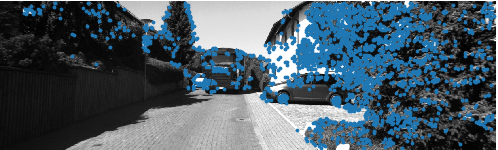
\includegraphics[width=\linewidth]{10_001157_001158_raw_corners_left}
    \caption{}
    \label{fig:ex_corner_and_matching:corner}
  \end{subfigure}
  \begin{subfigure}{.45\linewidth}
    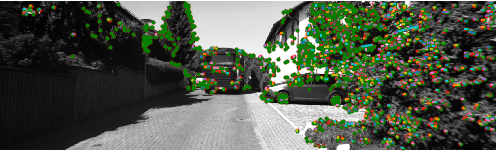
\includegraphics[width=\linewidth]{10_001157_001158_final_matches1}
    \caption{}
    \label{fig:ex_corner_and_matching:match}    
  \end{subfigure}
  \caption{Typical corner extraction and
    matching. Figure~\subref{fig:ex_corner_and_matching:corner} shows the raw
    extracted corners, while Figure~\subref{fig:ex_corner_and_matching:match} shows
    pruned and matched corners.}
  \label{fig:ex_corner_and_matching}
\end{figure}

\begin{figure}[!ht]
  \centering
  \begin{subfigure}{.45\linewidth}
    \centering
    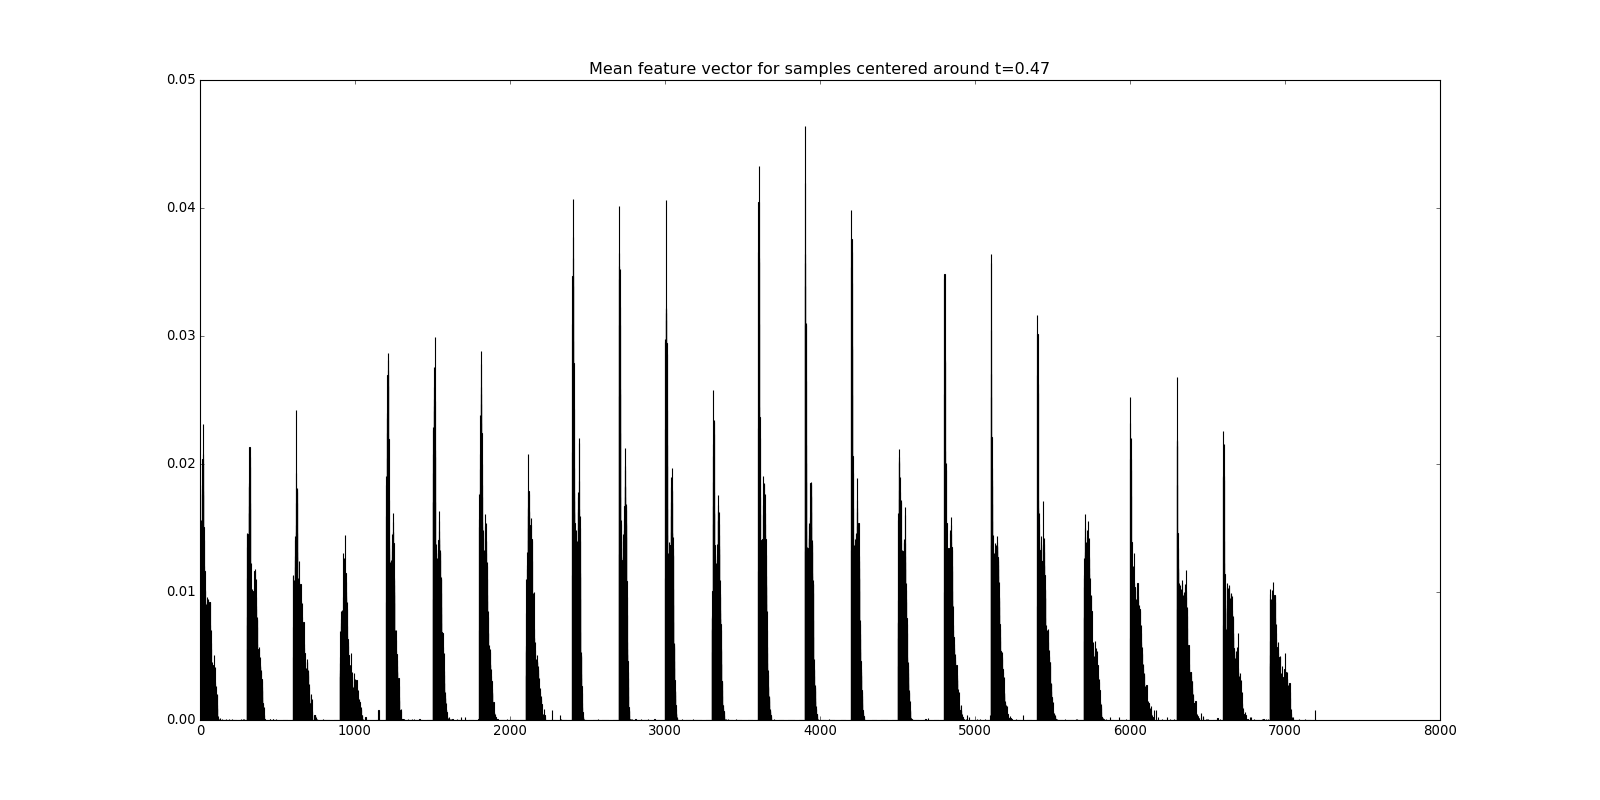
\includegraphics[width=1.2\linewidth]{00_mean_feature_vector_0_47}
    \caption{}\label{fig:1a}
  \end{subfigure}%
  \begin{subfigure}{.45\linewidth}
    \centering
    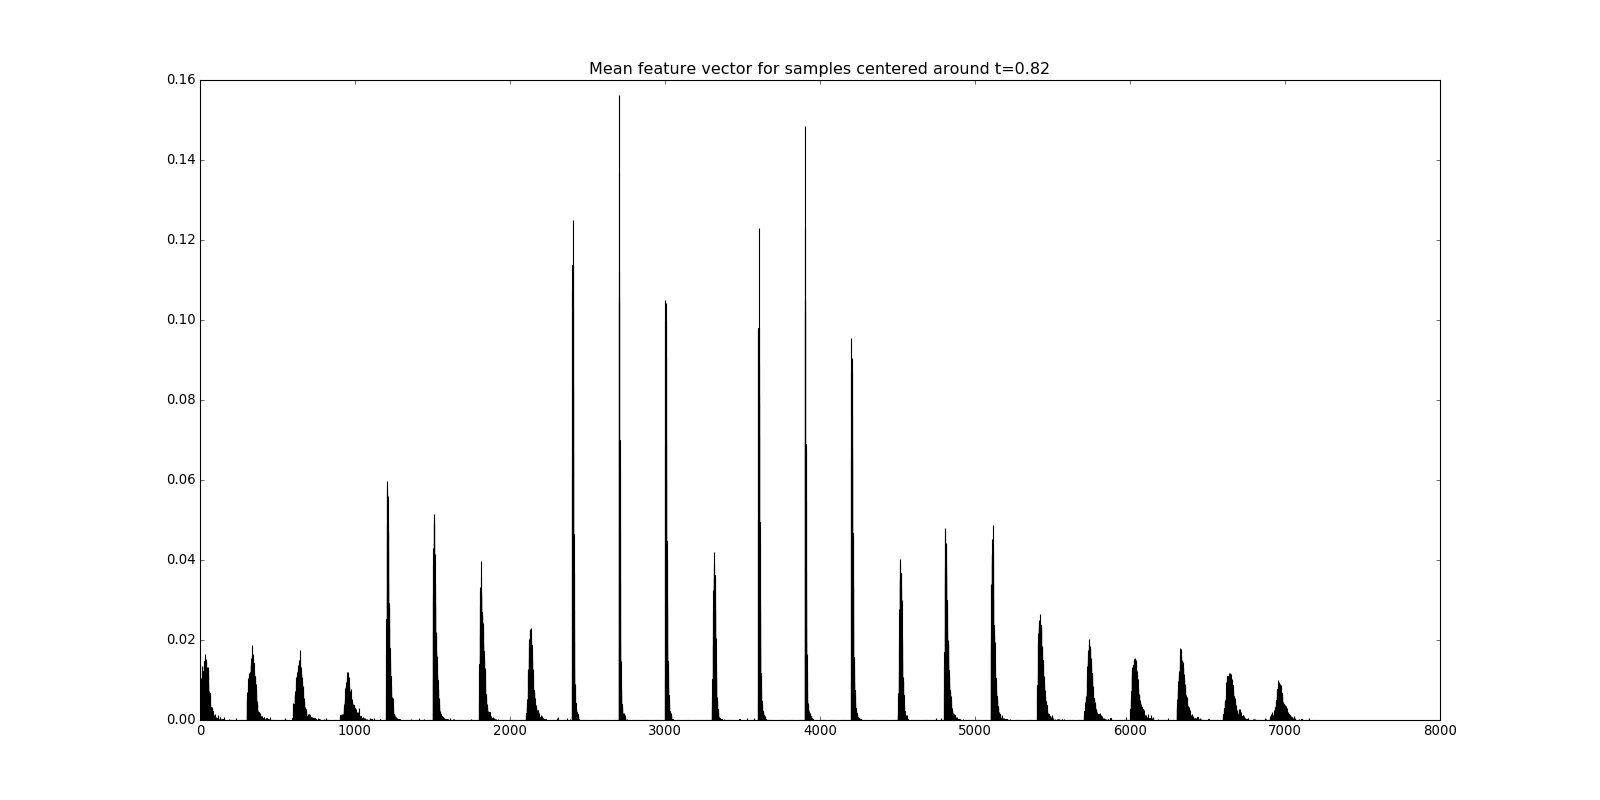
\includegraphics[width=1.2\linewidth]{00_mean_feature_vector_0_81}
    \caption{}\label{fig:1b}
  \end{subfigure}%
  \\
  \begin{subfigure}{\linewidth}
    \centering
    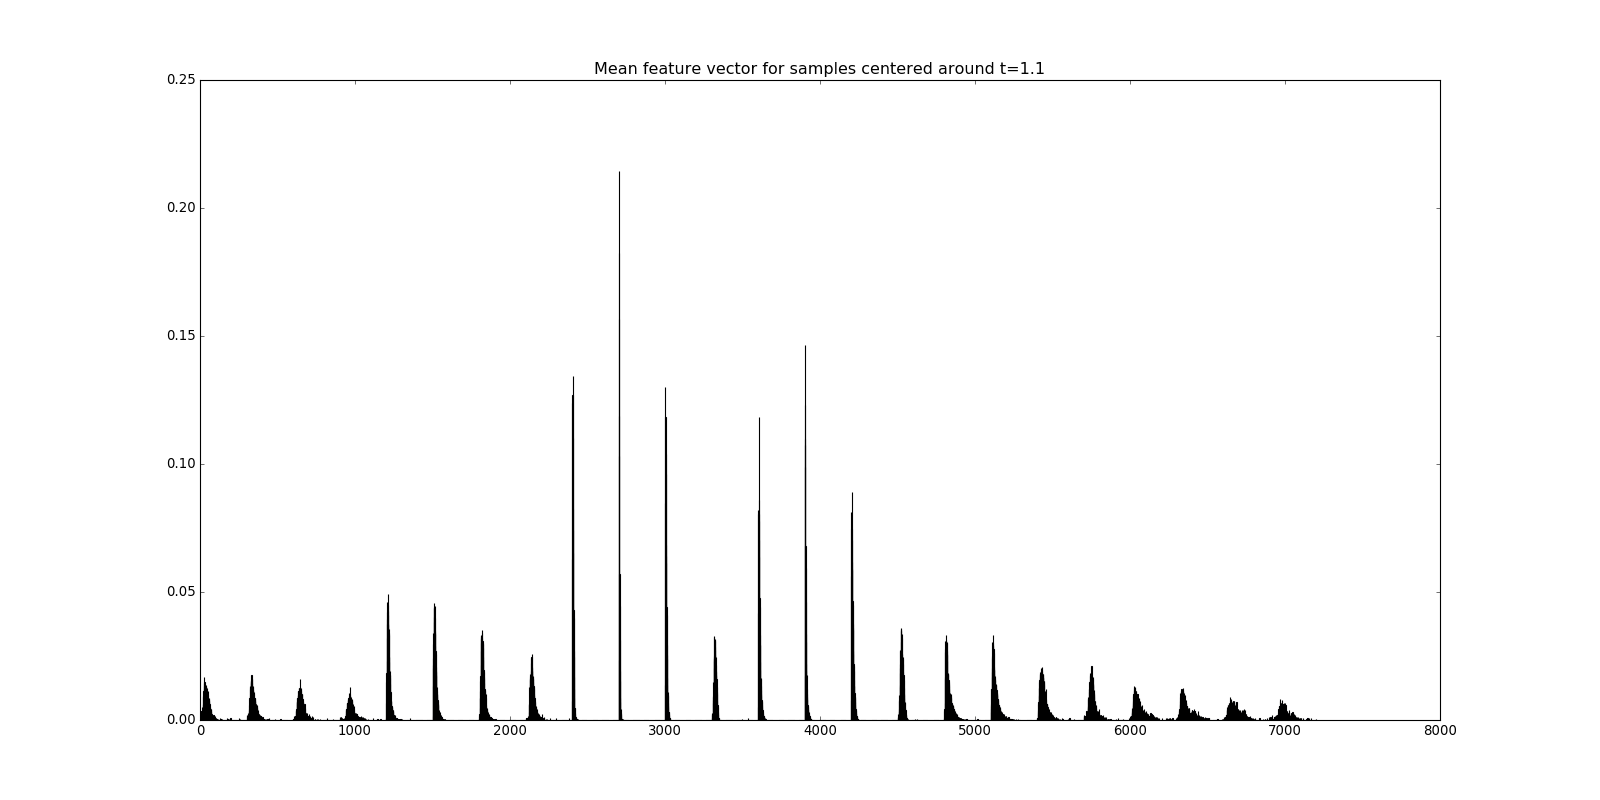
\includegraphics[width=.8\textwidth]{00_mean_feature_vector_1_1}
    \caption{}\label{fig:1c}
  \end{subfigure}%
  \caption{Average feature vectors for samples centered around the
    specific camera translation magnitude.  Each peak corresponds to a
    grid cell (e.g. here the grid is 4 rows by 6 columns by 300 bins,
    so the feature vector is of the dimension 6*4*300=7200).  The grid
    is sampled in a column-major mode. So the first four peaks
    correspond to the leftmost column of the image grid.}
  \label{fig:feature_vectors}
\end{figure}

We bin each image into $6\times 4$ grid.  For each bin in the image we
compute the histogram of corner disparities.  By disparity we denote
the displacement of the corner in the image.  We use $300$-bin
histogram for disparities (e.g, feature vector length is $7200$).

We use the extracted features to fit a random forest, by means of
recursive note splitting with sub-node variance minimization. The mean
absolute error is 0.174 meters with a standard deviation of 0.148
meters.

\section{Neural networks}

We use Caffe~\cite{jia2014caffe} framework to train and test our
models.
\paragraph{ZF} We train using vanilla SGD for 100 epochs and decrease
learning rate by factor of .1 every 10 epochs. We train the network
from scratch.
\paragraph{FlowNet} We also train using vanilla SGD for 100 epochs
decreasing learning rate by .1 every 10 epochs.  We start from
pre-trained weights of~\cite{fischer2015flownet}.
\paragraph{LSTM} TBD

\section{Results}

Let the ground truth sequence of camera motion scales by
$\{y_i\}_{i=0}^N$.  Let the predicted scales for the same sequence be
$\{\hat{y}_i\}_{i=0}^N$.  We report the mean absolute error:
\[
  \mu = \frac{1}{N}\sum_0^N{|y_i - \hat{y}_i|}
\]

\begin{table}[ht]
  \centering
  \begin{tabular}{ lcccc }
    \hline
                        & Random Forest & ZF   & FlowNet & LSTM ZF \\
    \hline
    $\mu\quad[meters]$        & .237          & .200 & \textbf{.103}    & .198 \\
    $\sigma\quad[meters]$     & .229          & .161 & \textbf{.08}     & .147 \\    
    \hline
  \end{tabular}
  \caption{Experimental Results}
  \label{table:1}
\end{table}


%%% Local Variables:
%%% mode: latex
%%% TeX-master: "../thesis"
%%% End:

\chapter{Conclusion}

This work treats two related sub problems in the field of vision aided
navigation.

The first part is of geometric nature and attempts to provide a new
insight into stereo and monocular motion estimation.  We show that if
one is able to split the image points into disjoint sets of near and
distant points, then we provide an estimation procedure for camera
motion.  Our algorithm is local by design and compares favorably to
its baseline.  By local we mean, that it does not build a map of the
environment and thus all its decisions are based on a pair of frames
that it sees.  Of course, there are larger SLAM systems that give
better accuracy overall.  Our algorithm may be used as a building
block of such systems or may be applicable in the compute-restrained
environment.

The second part of our work takes a statistical machine learning
approach, which leverages available data and compute power to solve
the visual navigation scaling problem.  We show how to train a model
to provide unbiased and low-variance scale estimates.  We also show a
simple approach which uses our scale estimates to provide full 6-DOF
motion estimation.  The work of~\cite{frost2017using} show a
different, more complex way to do motion estimation based on similar
scale estimates.  While the current result allows for scale drift free
motion estimation we feel that it may be greatly improved by better
use of the available data.

In recent years the field of visual navigation has matured
research-wise. It seems that most of the important fundamental
questions are answered.  Said that, there still is a significant gap
between state of the art and real world systems that rely on visual
data.  Part of this gap is in engineering, which is complex (most real
world systems use additional modalities: lidars, depth sensors,
etc.). We speculate that another part of the gap is that in order to
navigate in complex (e.g., urban) environments one can not rely on
geometric information alone and semantic understanding of the scene is
needed.

It also seems that the field is ready to take on larger-scale
problems, such as motion estimation and mapping on a very large scale,
collaborative large-scale mapping and navigation.  We feel that (at
least near-future) algorithms should leverage the power of traditional
geometry based approaches with a more recent data-driven methods.

One thing that we find very important is the appearance of new and
more challenging data sets.  KITTI, while being a great dataset is low
in its lighting, weather conditions, scenery and traffic variability.
We hope that the recent spree of the autonomous driving companies will
lead to the appearance of such new datasets, which in turn, will
foster new research.

%%% Local Variables:
%%% mode: latex
%%% TeX-master: t
%%% End:

% 
% Add any appendices here; they must come _before_ the bibliography
%
% \appendix
%\noappendicestocpagenum
%\addappheadtotoc
% 
\chapter{Some sort of an appendix}
\label{appendix:somesort}

You may want to include appendices of your own volition. Also, if you've developed any computer software, that needs to go in as an appendix as well.

\section{A section}

Some appendix content here. And something nice to finish things off:

\begin{figure}[htb]
  \centering
  \includegraphics[width=0.3\textwidth]{graphics/mygraphic2.png}
  \caption{A Flower.}
\end{figure}



% Back Matter
% ------------

% The following command will typeset the bibliography,
% then typeset the Hebrew part of the thesis:
% - Cover page
% - Title page
% - Acknowledgements page
%  (NO table of contents or list of figures in Hebrew)
% - (Extended) abstract (1000-2000 words)
%
% based on information you've provided in the thesis-fields file
% (including the relative paths to your bib files). The Hebrew
% content will be typeset in _reverse_page_order_, i.e. first
% in the file will be the last page of the abstract, and the
% Hebrew cover page will be the last page of the file.
%
\makebackmatter

% The resulting PDF can be printed and taken straight to binding,
% i.e. you do not need to flip any pages anywhere. Of course,
% mind the LaTeX error and warning messages, overfull hboxes etc.

\end{document}


%%% Local Variables:
%%% mode: latex
%%% TeX-master: t
%%% End:
